\chapter{CTMQC applied to the Tully Models}
\label{chap:tully_models}

The Tully models, first proposed by John Tully in 1990 \cite{tully_molecular_1990}, are a collection of simple 1 dimensional model systems. They were designed to be simple enough to obtain accurate quantum results to benchmark new nonadiabatic molecular dynamics (NAMD) methods against. Originally there were 3, 1 dimensional, 1 atom models. However, in this work an extra model has been introduced with parameters taken from Gossel \cite{gossel_coupled-trajectory_2018}. This is to allow a full comparison of my implementation of CTMQC with the literature. In this chapter my implementation of CTMQC will be tested using these model systems and by comparing my results with those in the literature.
\\\\
In each of the Tully models the (diabatic) Hamiltonian is a function of nuclear positions and is a 2$\times$2 matrix that takes the form:
\begin{equation}
  \hat{H} = \frac{\ \hat{P} ^2}{2M} + \left(
                                              \begin{array}{cc}
                                                H_{11}(\mathbf{R}) & H_{12}(\mathbf{R}) \\
                                                H_{21}(\mathbf{R}) & H_{22}(\mathbf{R})
                                              \end{array}
                                         \right)
\end{equation}
The nuclear mass has been set to 2000 a.u.. This was set to be very close to the proton's mass of 1836 a.u. so we can expect significant quantum effects that classical theory couldn't replicate. The values of the Hamiltonian matrix elements are set to produce systems that resemble common features in a typical nonadiabatic simulation such as avoided crossings and regions of extended coupling. The parameters used in each systems' Hamiltonian where taken from Gossel \cite{gossel_coupled-trajectory_2018} in order to compare the 2 implementations. These can be found in appendix \ref{ap:tully_params}.
\\\\
In order to propagate dynamics in the adiabatic basis we need to calculate various quantities from the hamiltonian at each timestep. These are, for Ehrenfest, the (adiabatic) nonadiabatic coupling vector ($\mathbf{d}_{lk}^{(I)}$) and the adiabatic energies ($E_{l}^{(I)}$). In the full CTMQC simulations we must also calculate the adiabatic momentum term $\mathbf{f}_{l}^{(I)}$ from the Hamiltonian. The adiabatic energies are the eigenvalues of the Hamiltonian. The adiabatic NACV can be calculated via a finite difference method and equation \eqref{eq:NACV_def} below.
\begin{equation}
  \mathbf{d}_{lk}^{(I)} = \langle \psi_{l}^{(I)} | \nabla \psi_k^{(I)} \rangle
  \label{eq:NACV_def}
\end{equation}
Where $\psi_{l}^{(I)}$ is the adiabatic electronic basis function for adiabatic state $l$. This is given by the eigenvector of the Hamiltonian, on replica $I$, corresponding to state $l$. Illustrations of these 2 properties can be found below in fig \ref{fig:tully_schematics} for each of the 4 models systems.
\begin{figure}[H]
  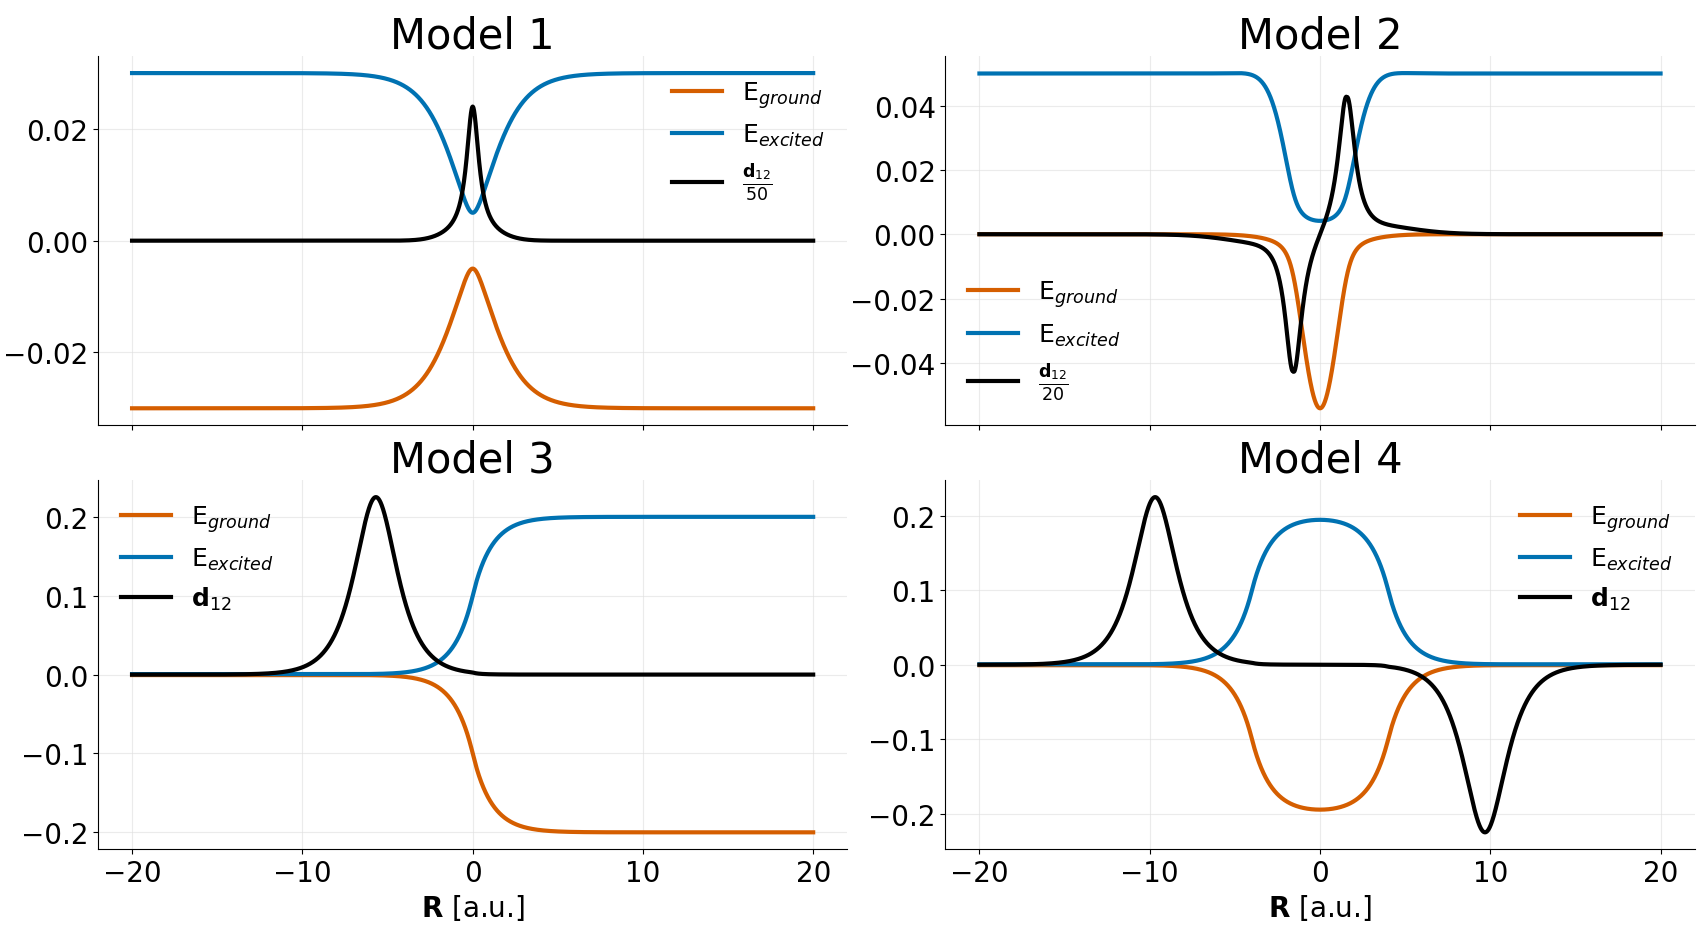
\includegraphics[width=\textwidth]{Chapter_tullyModels/model_schematics.png}
  \caption{\label{fig:tully_schematics}Adiabatic potential energy surfaces (orange and blue) and element 1, 2 of the nonadiabatic coupling vector (black) for the 4 model systems. For parameters see appendix \ref{ap:tully_params}.}
\end{figure}
\newpage
\noindent In order to initialise the simulations coordinates and velocities were sampled from the Wigner phase-space distribution of a gaussian nuclear wavepackets given by equation \eqref{eq:initial_nucl_wp}. A derivation of this can be found in appendix \ref{ap:Wigner}. The nuclear positions/velocities were then propagated using a velocity verlet algorithm and the adiabatic expansion coefficients were propagated using a 4$^{th}$ order Runge-Kutta method.
\begin{equation}
  \chi(R, 0) = \frac{1}{(\pi \mu^2)^{\frac{1}{4}}} e^{-\frac{(R - R_0)^2}{2 \mu^2} + \im k_0 (R - R_0) }
  \label{eq:initial_nucl_wp}
\end{equation}
The adiabatic coefficients were initialised purely on the ground state and the initial width of the nuclear wavepacket was set to $\mu = \sqrt{2}$ bohr. 2 values of initial momenta $k_0$ were chosen for each model, 1 low value and another higher one. Full details of all input parameters can be found in appendix \ref{ap:tully_params}. I have implemented a serial version of CTMQC acting on Tully's toy model systems and real molecular systems using couplings derived from the analytic overlap method \cite{gajdos_ultrafast_2014} within the software package CP2K \cite{cp2k} and for Tully's model systems as standalone python code. These are accessible publicly via github repositories at: \href{https://github.com/95ellismle}{github.com/95ellismle}. This work will only focus on results from the CP2K implementation as we will later see this code extended and applied to systems of real Ethylene molecules.

\section{Testing My Implementation -Ehrenfest}
The motivation behind implementing CTMQC for the Tully models was to serve as a verifiable base for later extensions, such as integrating CTMQC within the fragment-orbital based (FOB) \cite{spencer_fob-sh:_2016} framework which will be discussed in a later chapter \ref{chap:molecular_systems}. Using such simple systems will also help to clarify how each new parameter works and make testing and debugging easier. As well as many numerical tests on individual terms in the equations,  I have implemented some physical tests on the overall system dynamics. In this section, I will outline the key tests I have performed on the Ehrenfest propagation and will include the full details of the full CTMQC propagation in the following section.
\\\\
In all the simulations when the Tully models are referenced they will refer to those parameters given in appendix \ref{ap:tully_params}. Reference to a high momentum Tully model simulation is a reference to that model with initial momenta being sampled from the Wigner distribution of the higher of the 2 initial momenta given in appendix \ref{ap:tully_params}.

\subsection{Norm Conservation}
\label{sect:normConsEhren}
\begin{figure}[ht]
	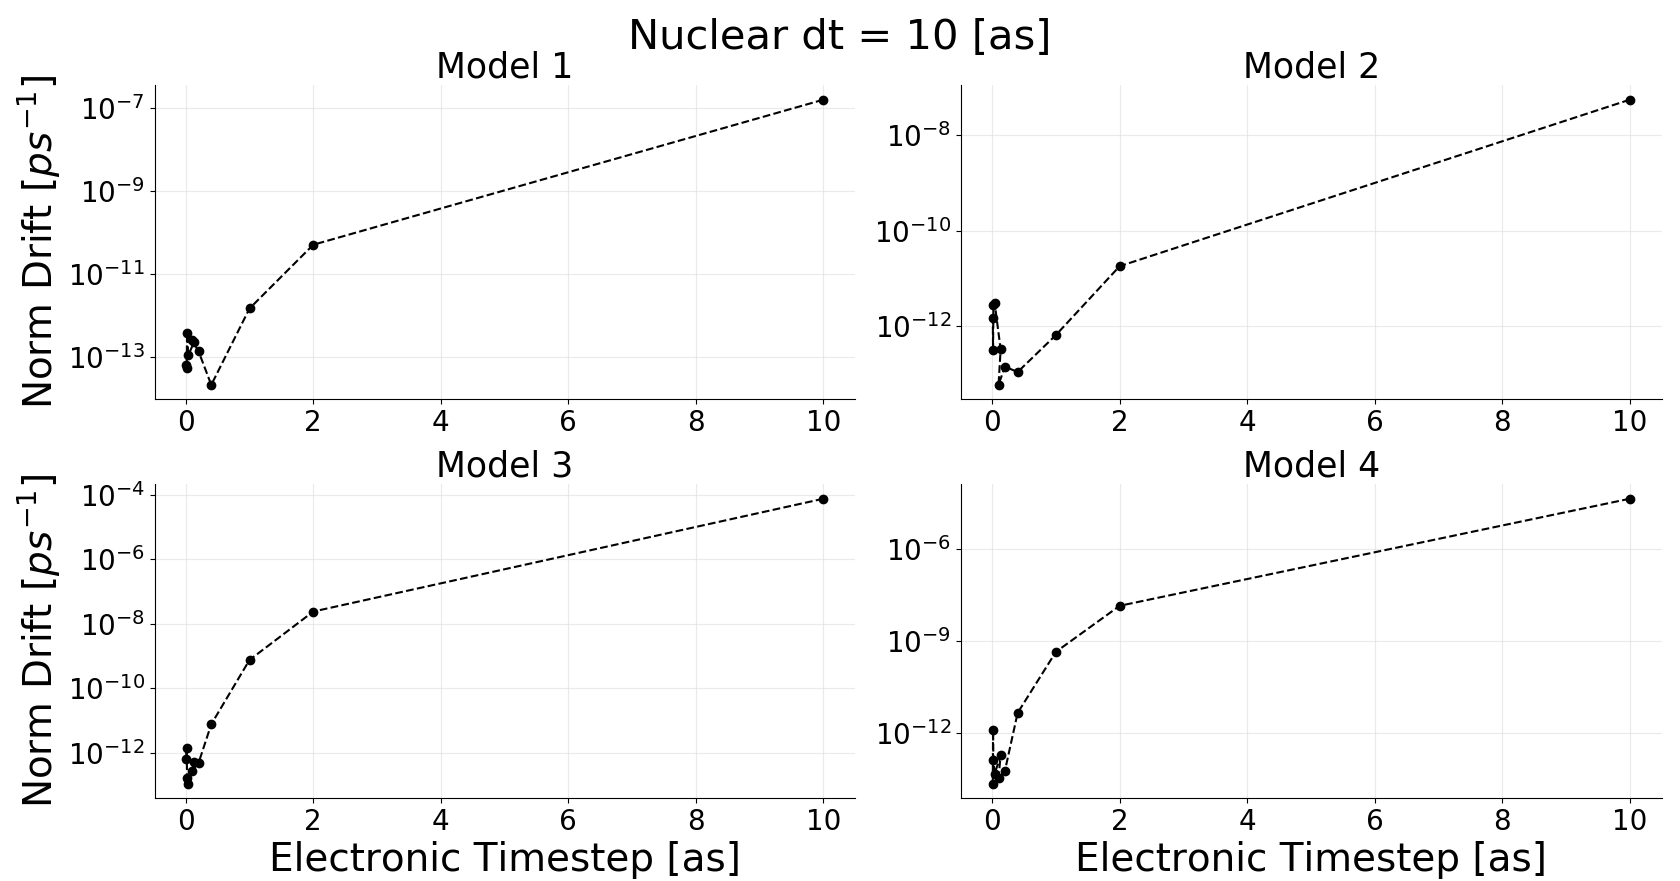
\includegraphics[width=\textwidth]{/home/matt/Documents/PhD/PhD_Thesis/img/CTMQC/TullyModels/Ehren_Norm_Conservation.png}
	\caption{\label{fig:EhrenNormCons}The norm conservation averaged over all replicas for Ehrenfest simulations with various electronic timesteps for each Tully model using a initial high momenta.}
\end{figure}
\noindent In appendix \ref{ap:norm_cons}, it is shown that the norm of the adiabatic expansion coefficients should be conserved throughout the simulation. To test the conservation of the norm of the expansion coefficients Ehrenfest simulations were ran with various electronic timesteps (with a constant nuclear timestep) for each of the 4 high momentum Tully models. The high momentum Tully models were chosen as they are expected to provide a worst case scenario of the norm conservation, due to populations changing more quickly leading to reduced sampling. As can be seen in figure \ref{fig:EhrenNormCons}, the norm of the wavefunction is conserved within numerical error ($10^{-12}$) when     using a sufficiently small timestep in every Tully model.

\subsection{Energy Conservation}
Energy conservation is a very important property in most molecular dynamics simulations. In Ehrenfest of mean-field molecular dynamics nuclei are propagated on a population-weighted mean potential energy surface, e.g. $\sum_{k}|C_{l}^{(I)}(t)|^2 = E_{eff}(t)$ \cite{EhrenEnerCons}. Kinetic energy of the classical nuclei is given by the standard formula, e.g. $\frac{1}{2} m v^2$. We can therefore write down the conserved quantity as defined below in equation \eqref{eq:EhrenfestEnergyConservation}:
\begin{equation}
  \frac{d E}{dt} = \frac{d}{dt} \left[ \frac{1}{2} m v^2 + \sum_{k}|C_{l}^{(I)}(t)|^2 \right] = 0
  \label{eq:EhrenfestEnergyConservation}
\end{equation}
As in the norm conservation checks in section \ref{sect:normCons},  parameters from the high momentum cases were taken as initial conditions for simulations with various nuclear timesteps, this time holding the electronic timestep constant. The high momenta cases were chosen to show the worst case energy conservations. A linear line of best fit was then fitted to the data and the drift in the total energy (given in \eqref{eq:EhrenfestEnergyConservation}) was calculated from its gradient. The results of these simulations are given in figure \ref{fig:EhrenEnerCons}.
\begin{figure}[ht]
  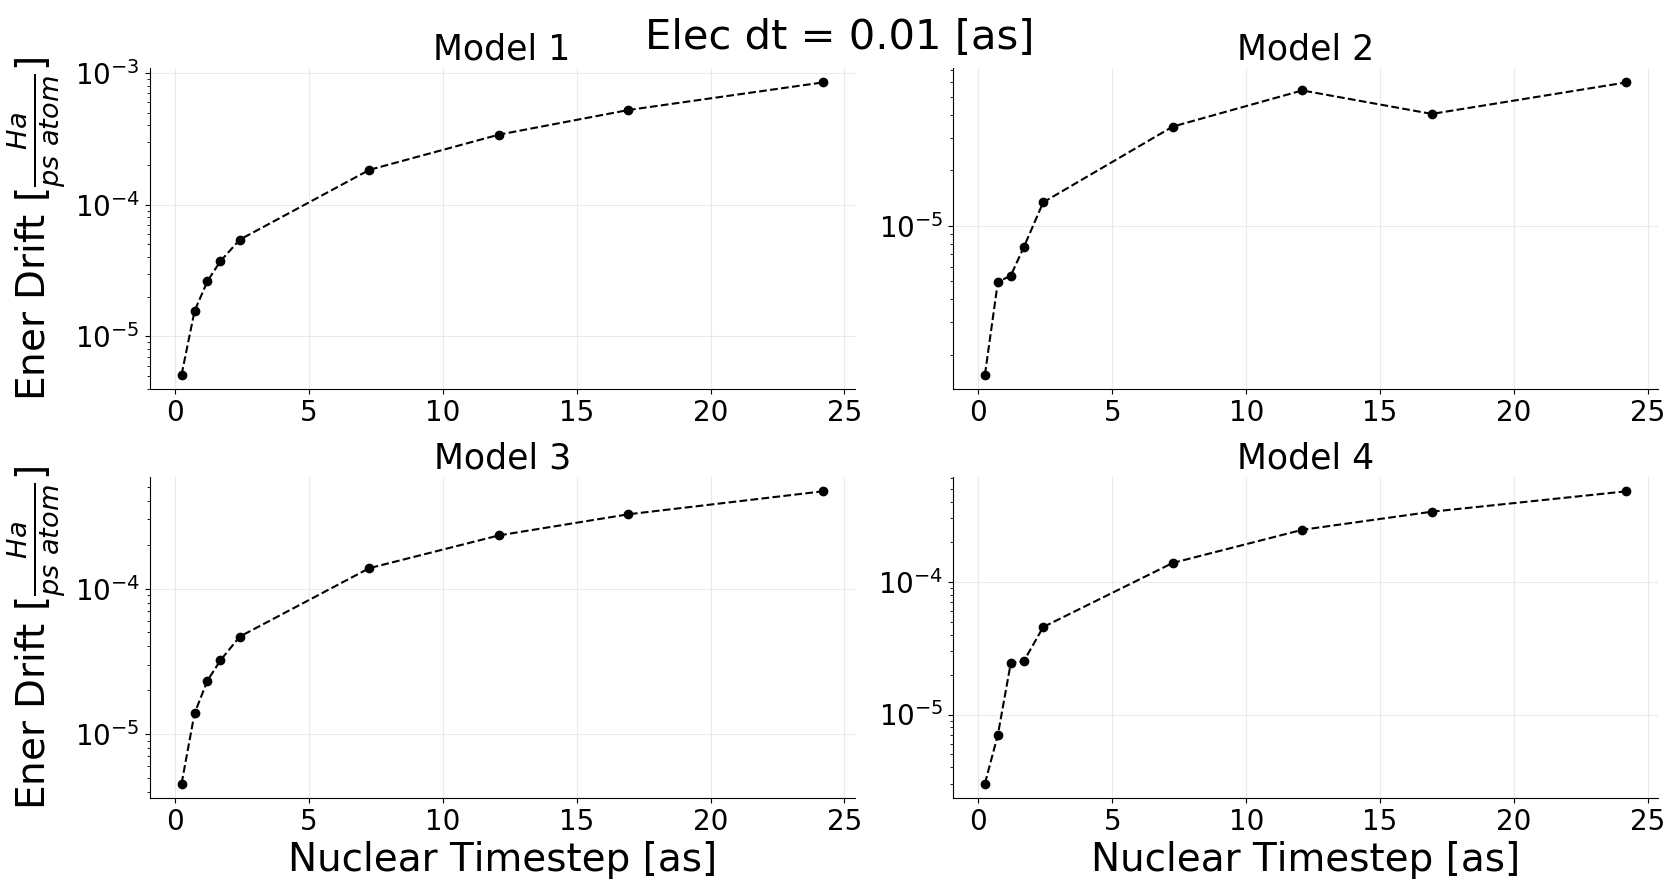
\includegraphics[width=\textwidth]{./img/CTMQC/TullyModels/Ehren_EnerCons.png}
  \caption{\label{fig:EhrenEnerCons}Energy conservation values for various nuclear timesteps for the high momentum case of each Tully model using Ehrenfest dynamics.}
\end{figure}
In figure \ref{fig:EhrenEnerCons}, we see the expected results that as the nuclear timestep is decrease the drift in the total energy also decreases. This is due to increased sampling of atomic movements leading to more continuous forces being calculated. This trend validates the implementation and shows that in the limit of infinitely small timestep (and infinite computer precision) perfect energy conservation would be achieved. However, fairly small nuclear timesteps are required to achieve reasonable energy conservations. This is because the system contains only 1 atom with a mass comparable to that of Hydrogen. If one needed an improved energy conservation a higher order integrator than the velocity verlet used here may also improve results slightly.

\subsection{Comparisons To Literature}
\subsubsection{Gossel and Agostini}
\label{sect:EhrenCompare}
There have been 2 papers published applying CTMQC and Ehrenfest to the Tully models \cite{gossel_coupled-trajectory_2018, agostini_quantum-classical_2016} and both contain results for the 4 Tully models shown in fig \ref{fig:tully_schematics}. The results contain data on the (ground state) adiabatic populations and a coherence indicator (shown in equation \eqref{eq:coherence_indicator}) for 16 different simulations (a low and high initial momentum simulation of Models 1, 2, 3 and 4). However, models 1 and 4 in Agostini \cite{agostini_quantum-classical_2016} used a different initial momentum so these have been omitted from the results in figures \ref{fig:LitCompEhrenTullyLow} and \ref{fig:LitCompEhrenTullyHigh}. The adiabatic populations give the probability of find the wavefunction on a particular adiabatic state and their values can range from 0 $\rightarrow$ 1. A value of 1 means that the wavefunction is completely localised on 1 adiabatic state and there is a certainty of finding it there, and vice versa for 0. The coherence indicator gives an indication of how much `mixing' has occurred between adiabatic states and can have a value from 0 $\rightarrow$ 0.25. A value of 0 means that the adiabatic population has completely localised on just 1 state. A value of 0.25 means that the population is equally split between the 2 states.
\begin{equation}
	|\rho_{12}(t)|^2 = \frac{1}{N_{tr}} \sum_{I=1}^{N_{tr}} |C_{1}^{(I)}(t)|^2 |C_{2}^{(I)}(t)|^2
	\label{eq:coherence_indicator}
\end{equation}
\\\\
In order to compare to results in the literature the same setup had to be used. In this case this meant sampling individual replicas' initial conditions (positions and momenta) from a Wigner distribution with a mean position and momenta given in appendix \ref{ap:tully_params}. The wavefunction was initialised purely on the ground state and the same integrator was used for the nuclear and electronic propagation (velocity verlet and RK4 respectively).
\begin{figure}[ht]
	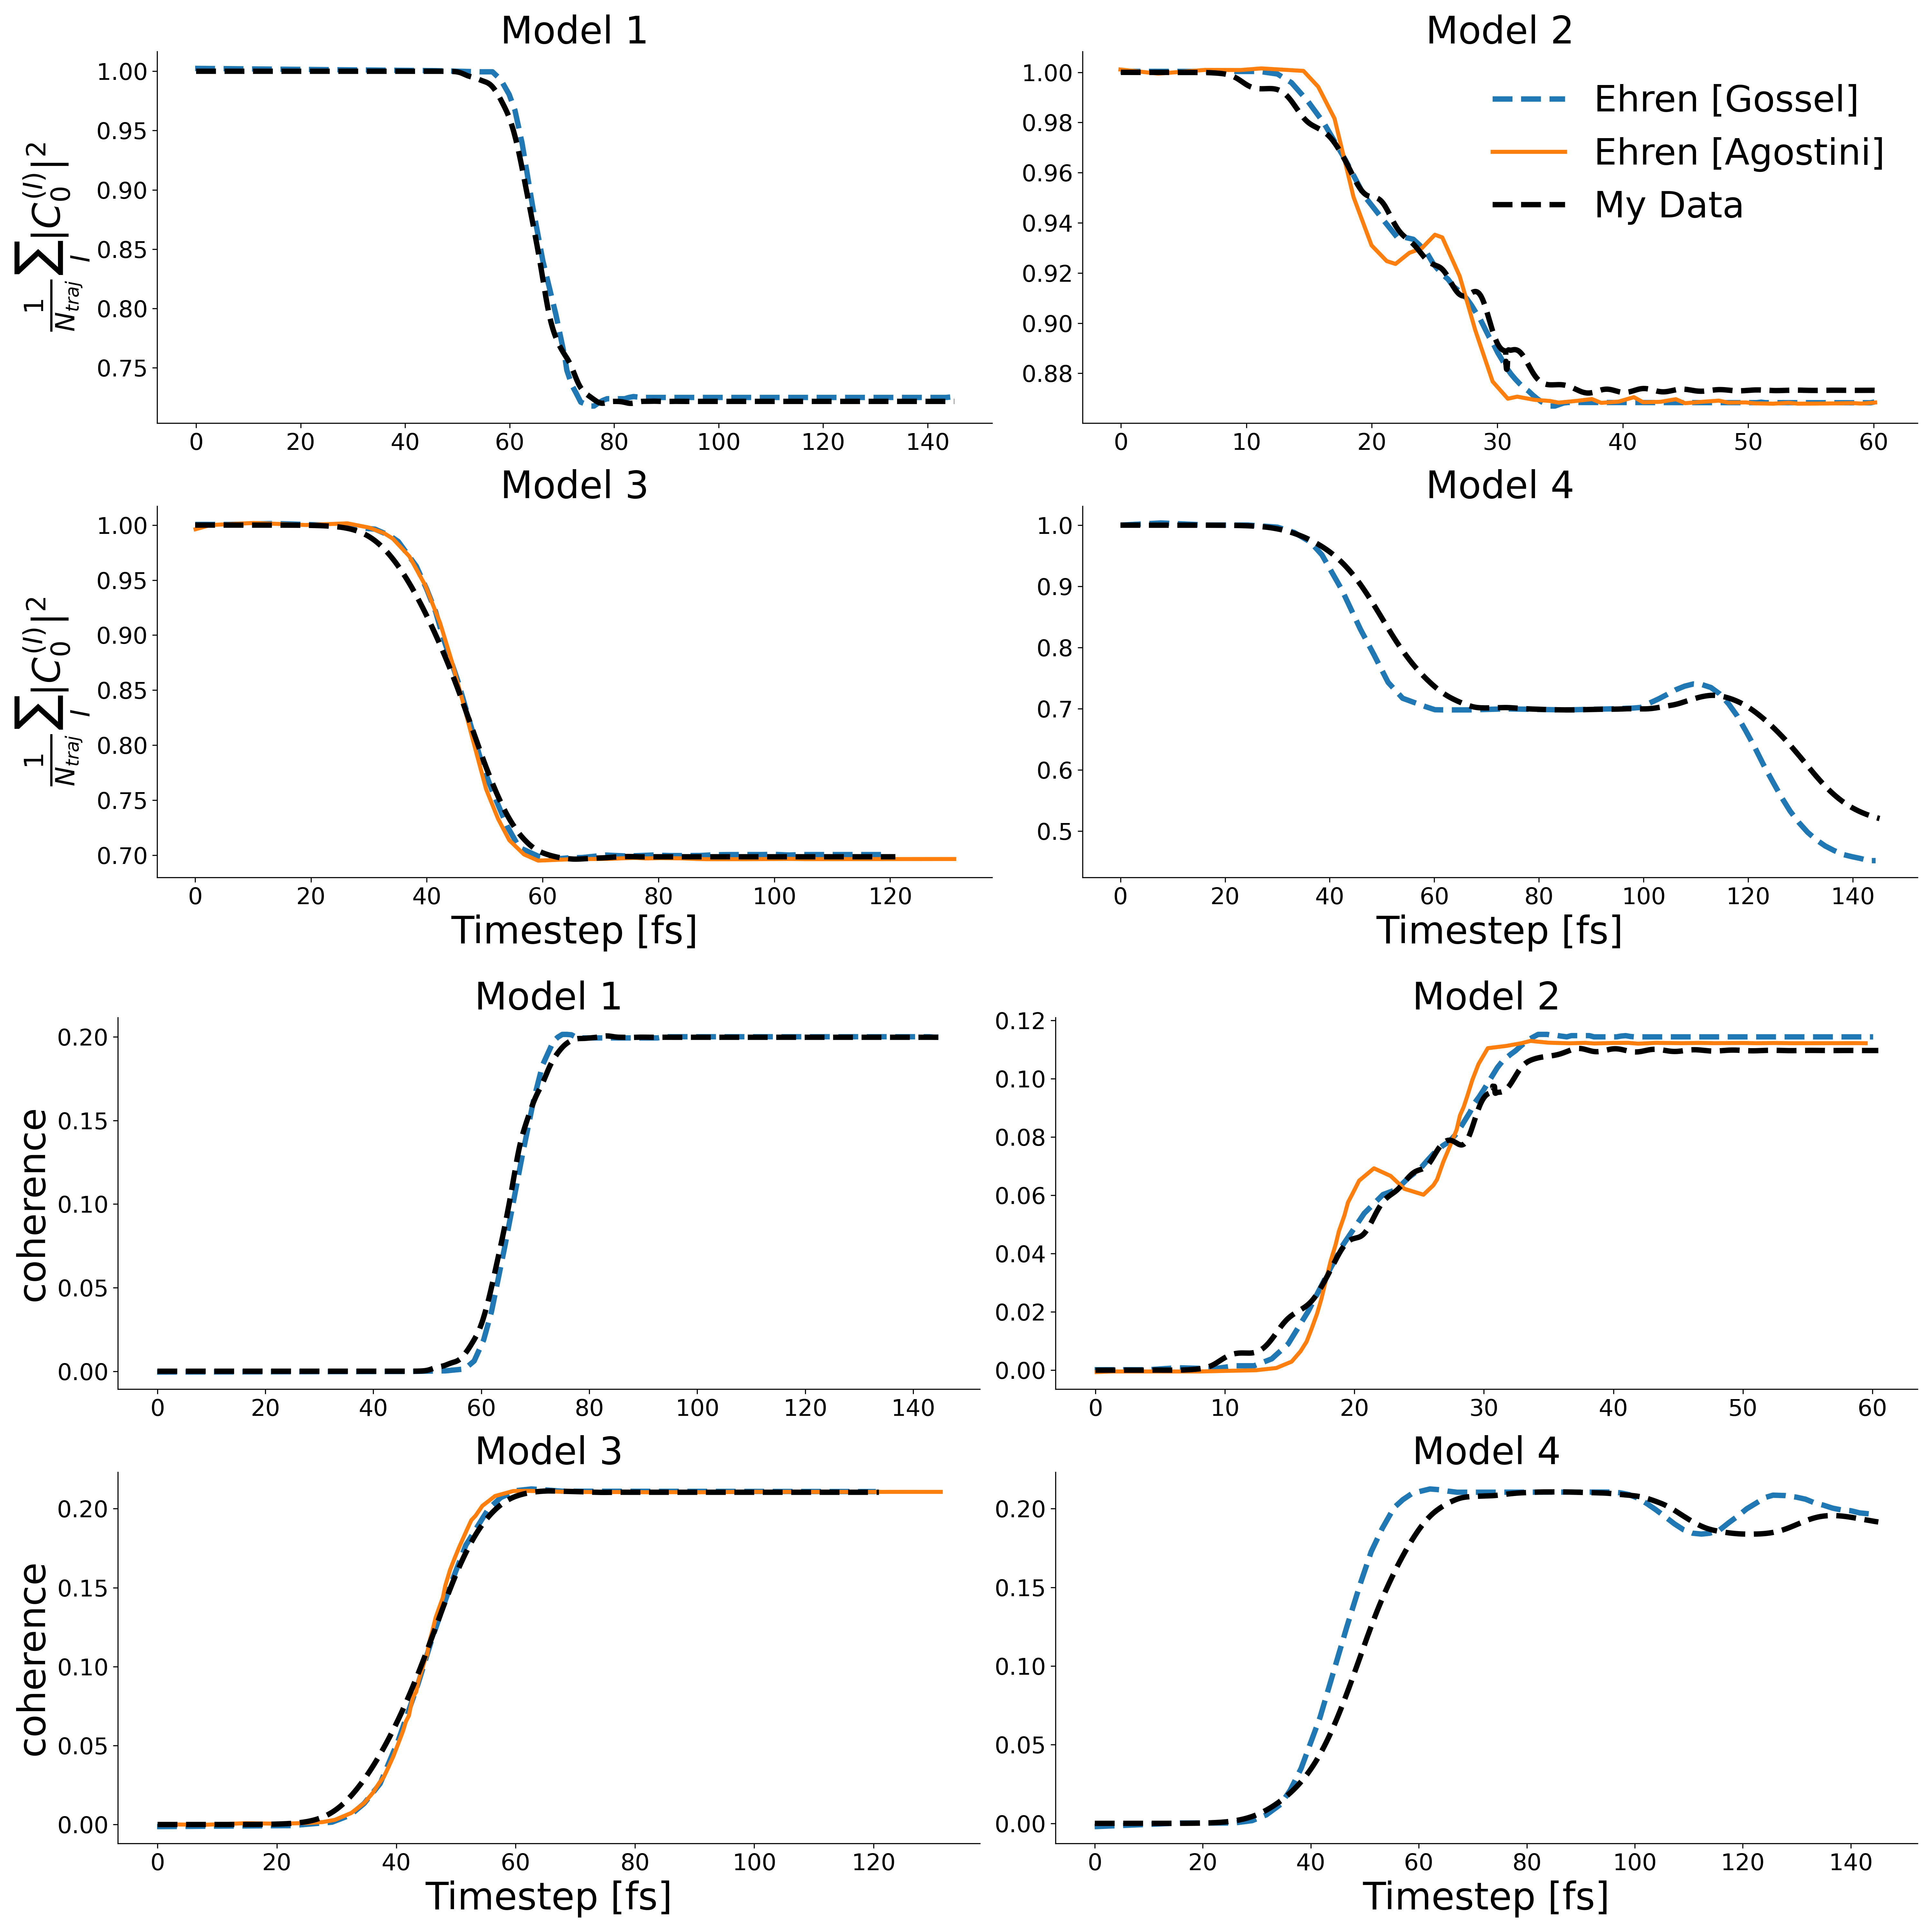
\includegraphics[width=\textwidth]{img/CTMQC/TullyModels/Ehren_lowMom.png}
	\caption{\label{fig:LitCompEhrenTullyLow}A comparison of my implementation of Ehrenfest (for 4 model Hamiltonians) and results from the literature for the low momenta cases. The black dashed lines show my data (ground state ad pops), the orange dashed lines are data from Agostini \cite{agostini_quantum-classical_2016} and the blue solid lines are from Gossel \cite{gossel_coupled-trajectory_2018}. The figures are labelled with their model number, whether the initial momentum was high or low and whether the populations or coherence indicator was plotted.}
\end{figure}
\begin{figure}[ht]
	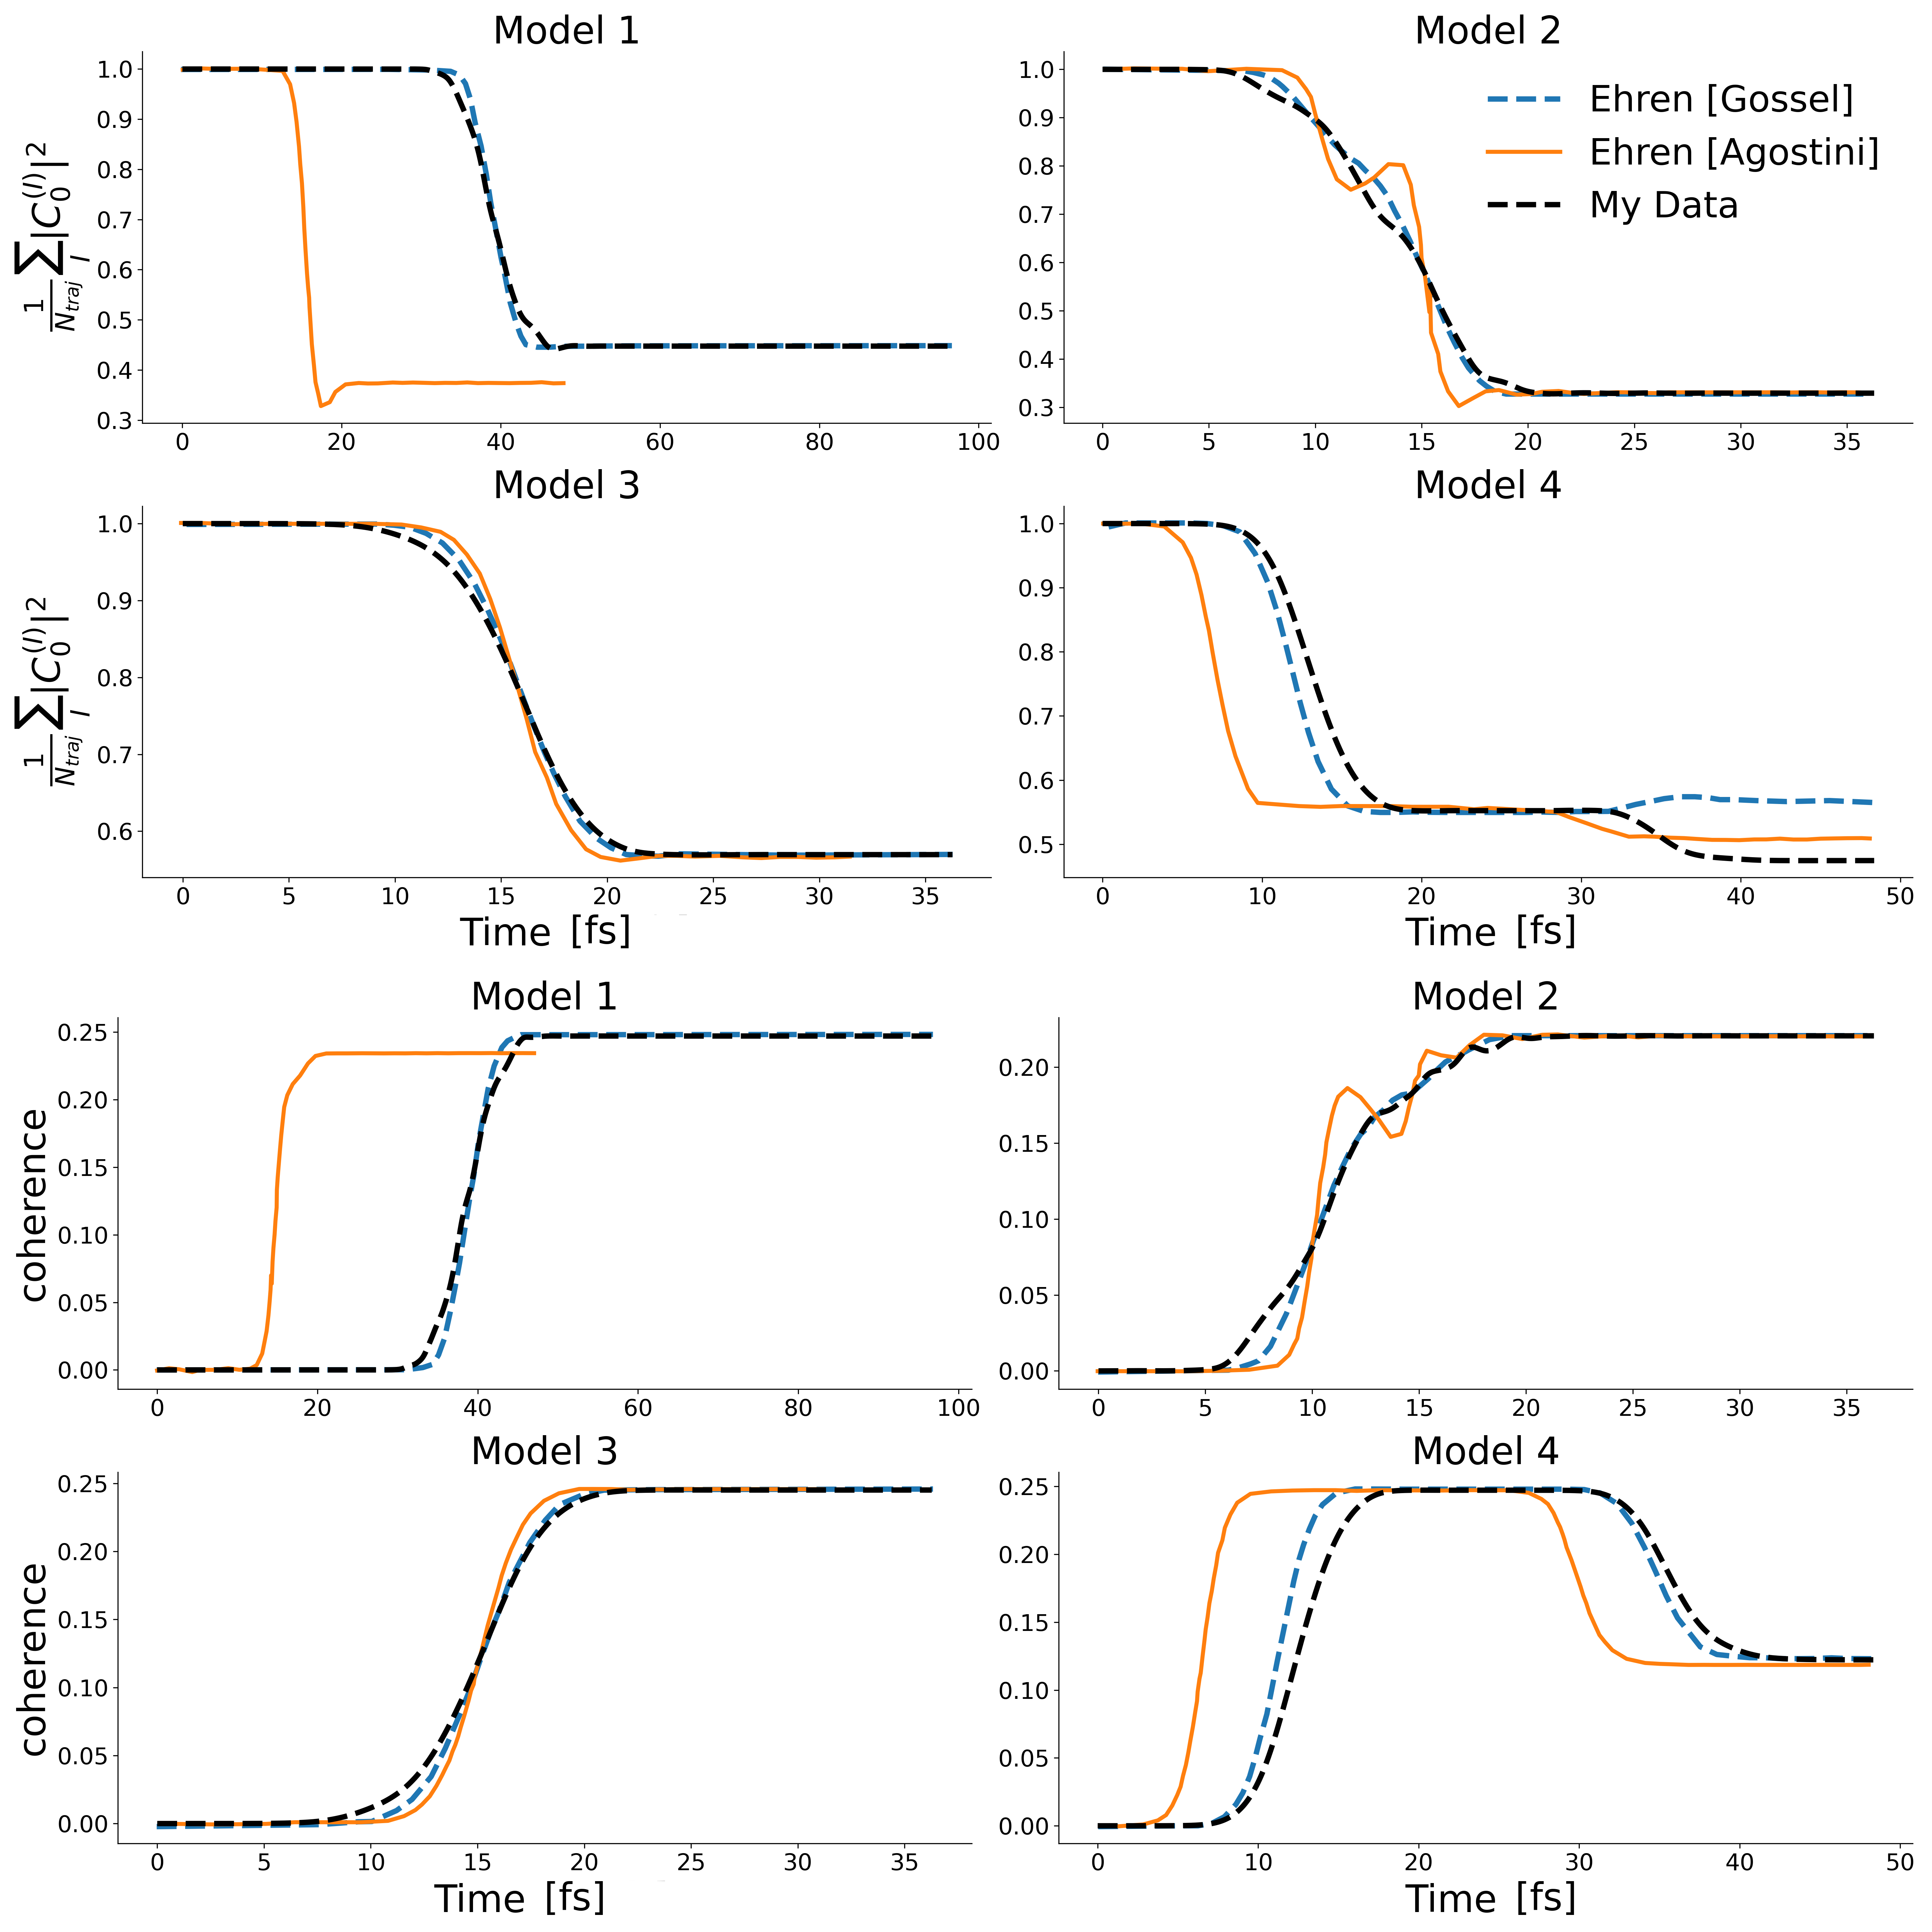
\includegraphics[width=\textwidth]{img/CTMQC/TullyModels/Ehren_highMom.png}
	\caption{\label{fig:LitCompEhrenTullyHigh}A comparison of my implementation of Ehrenfest (for 4 model Hamiltonians) and results from the literature for the high momenta cases. The black dashed lines show my data (ground state ad pops), the orange dashed lines are data from Agostini \cite{agostini_quantum-classical_2016} and the blue solid lines are from Gossel \cite{gossel_coupled-trajectory_2018}. The figures are labelled with their model number, whether the initial momentum was high or low and whether the populations or coherence indicator was plotted.}
\end{figure}
\noindent My results as well as the relevant data taken from Agostini and Gossel \cite{agostini_quantum-classical_2016, gossel_coupled-trajectory_2018} are shown in figures \ref{fig:LitCompEhrenTullyLow} (low momentum) and \ref{fig:LitCompEhrenTullyHigh} (high momentum) for Ehrenfest dynamics. This is equivalent to full CTMQC dynamics where the quantum momentum term is set to 0. Hence, we can test most parts of the code (i.e. Runge-Kutta propagation, velocity verlet, inputs, force calculations etc...) while ignoring the new quantum momentum and accumulated adiabatic force terms.
\\\\
The results in figures \ref{fig:LitCompEhrenTullyLow} and \ref{fig:LitCompEhrenTullyHigh} show that both the adiabatic populations and coherence indicator give exactly the same results as in the literature, within reasonable error. Any deviations of results come from either a slightly different initial sampling of positions or small errors in extracting data from the graphs in each of the papers. For example, in the case of the high initial momentum simulation of model 4 all 3 results show some differences though the trend is very similar. This is true also in the Model 2 results where the Agostini populations show some transient oscillations before settling onto the same equilibrium population. This may be due to a smaller spread of positions being used in the initial sample leading to similar oscillations that aren't smoothed out in the averaging over all replicas. There are also a couple of models that start at a slightly different initial mean position in Agostini \cite{agostini_quantum-classical_2016} thus they hit the nonadiabatic crossing region sooner. These are model 1 and 4 for the high momentum case.
\\\\
Although not all results are exactly the same, I believe the populations agree well enough within a reasonable error to serve as a confirmation of my implementation.
\subsubsection{Subotnik}
As a final confirmation of my implementation and an investigation of the underlying physics, in a Subotnik \cite{SubotnikMomentumEhrenfest}, results were published for Ehrenfest simulations carried out on the 3 original Tully Models. In this work, the author presented the probabilities of the population being found transmitted through the region of nonadiabatic coupling on the ground or excited state and the probability of being reflected on the ground or upper state. In the results below, I will show comparisons of just the transmission probability onto the ground state. That is, the population that travels on the ground state beyond the region of high nonadiabatic coupling. Other probabilities will not be shown in the interest of brevity, though they agree with the published results as well as the ground state transmission in figure \ref{fig:SubotnikComparison}.
\begin{figure}[ht]
  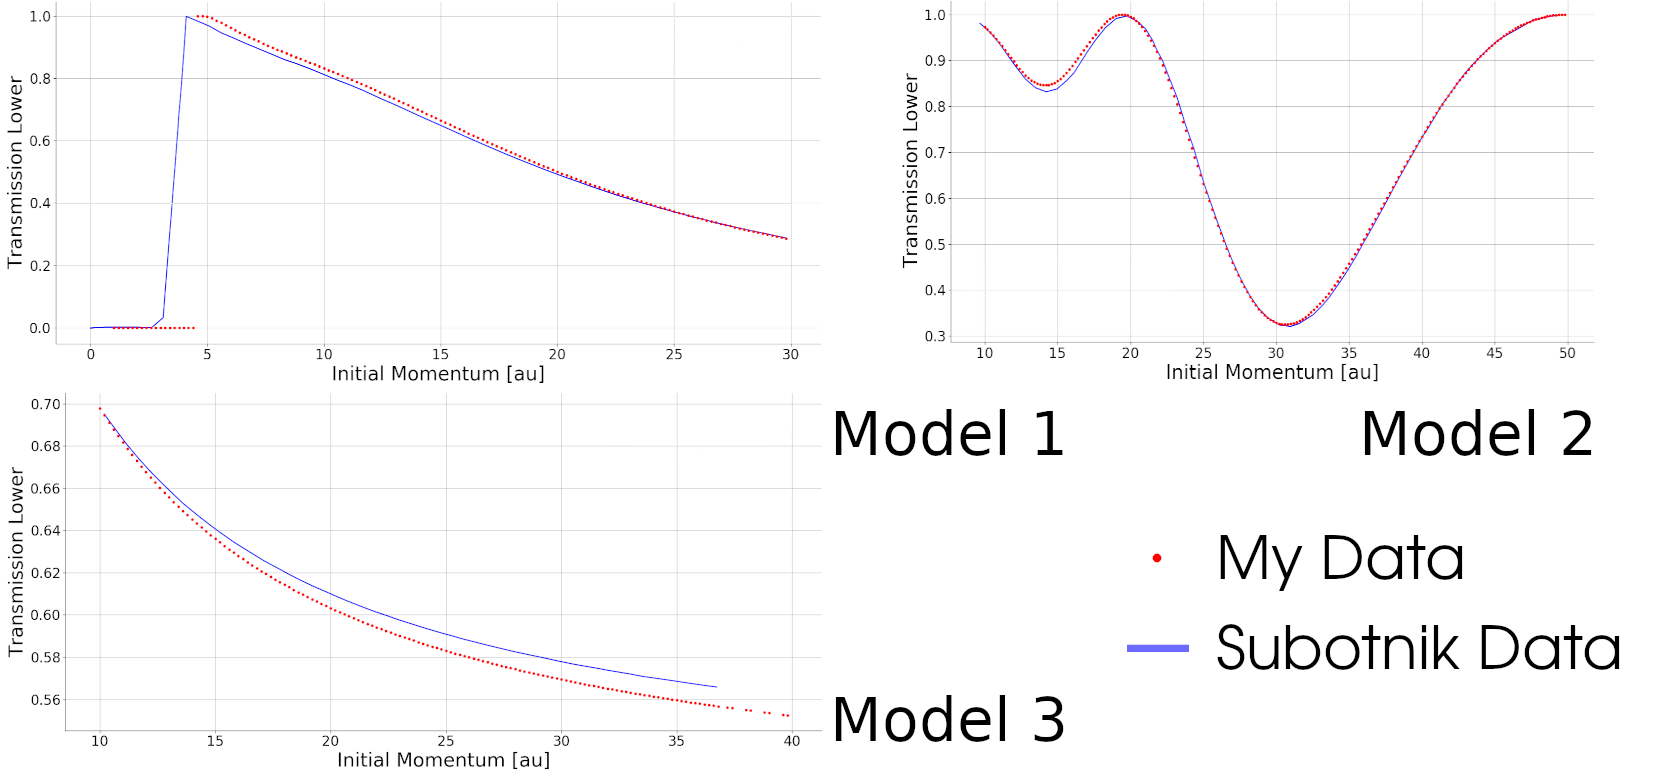
\includegraphics[width=\textwidth]{img/CTMQC/TullyModels/Ehrenfest_vs_Subotnik.png}
  \caption{\label{fig:SubotnikComparison}Comparison of transmission probabilities through the region of high nonadiabatic coupling on the ground state. Tully model 1 is shown in the top-left, Tully model 2 is shown in the top-right and Tully model 3 is shown in the bottom-left.}
\end{figure}
As can  be seen in figure \ref{fig:SubotnikComparison} my implementation of the Ehrenfest simulation code for the Tully models agrees very well with those in Subotnik \cite{SubotnikMomentumEhrenfest}. The small deviation (less than 1\% maximum disagreement) within each model is due to errors in retrieving data from images in original paper and possibly slightly different analysis methods. In model 1 (top-left pane) we see there is 0 ground state population transmission below an initial momentum of around 3-4 au. This is due to the fact that the nuclei do not have enough kinetic energy to make it over the potential hill (see figure \ref{fig:tully_schematics}) and never reach an area of high nonadiabatic coupling. The sharp cutoff is due to the classical treatment of the nuclei. In the original Subotnik \cite{SubotnikMomentumEhrenfest} paper exact results were given showing the slower decay to 0 transmission with respect to initial momenta. Beyond this initial activation momentum, increases to initial momentum results in lower ground state transmissions. This is because the system has more kinetic energy allowing a higher proportion of the wavefunction to be transmitted on the excited state.
\\\\
In model 2 we observe St\:uckelberg oscillations as the atom is forced through an avoided crossing twice. During the first pass through the avoided crossing some population transfer onto the excited state occurs. In the next passage through the avoided crossing the wavefunction, now split over 2 energy levels and travelling coherently, can interfere with itself. The type of interference is dependent on the velocity of the particle passing through the avoided crossings and varies in an oscillatory fashion as seen in figure \ref{fig:SubotnikComparison}.
\\\\
In model 3, as the particle approaches $\mathbf{R}=0$ it passes through a region of strong coupling, with a very small energy gap between energy levels. As the 2 energy levels diverge at $\mathbf{R}=0$ the nonadiabatic coupling dies down to 0 and the population remains trapped on the energy level it was on at $\mathbf{R}=0$. Increases in initial momentum of the particle increases the likelihood that we see the particle transmit on the excited state.
\\\\
These tests serve as a confirmation of the implementation of the Ehrenfest propagator. The full CTMQC equations can be implemented using the majority of the Ehrenfest infrastructure with extensions to account for the quantum momentum terms.

\section{Testing my implementation -CTMQC}
\subsection{Conservation of the norm}
In figure \ref{fig:CTMQCNormCons} only Model 3 shows a similar trend as in Ehrenfest for the norm conservation -i.e. a decreasing electronic timestep gives a rapidly decreasing norm drift. In models 1 and 2 we see that the norm drift doesn't get much better as we decrease the timestep and there are large error bars associated with each data point. In model 4 this is less pronounced but is still clearly affected. This is due to an instability in the current formalism of the quantum momentum term ($\mathcal{Q}_{lk, \nu}^{(I)}$).
\begin{figure}[ht]
	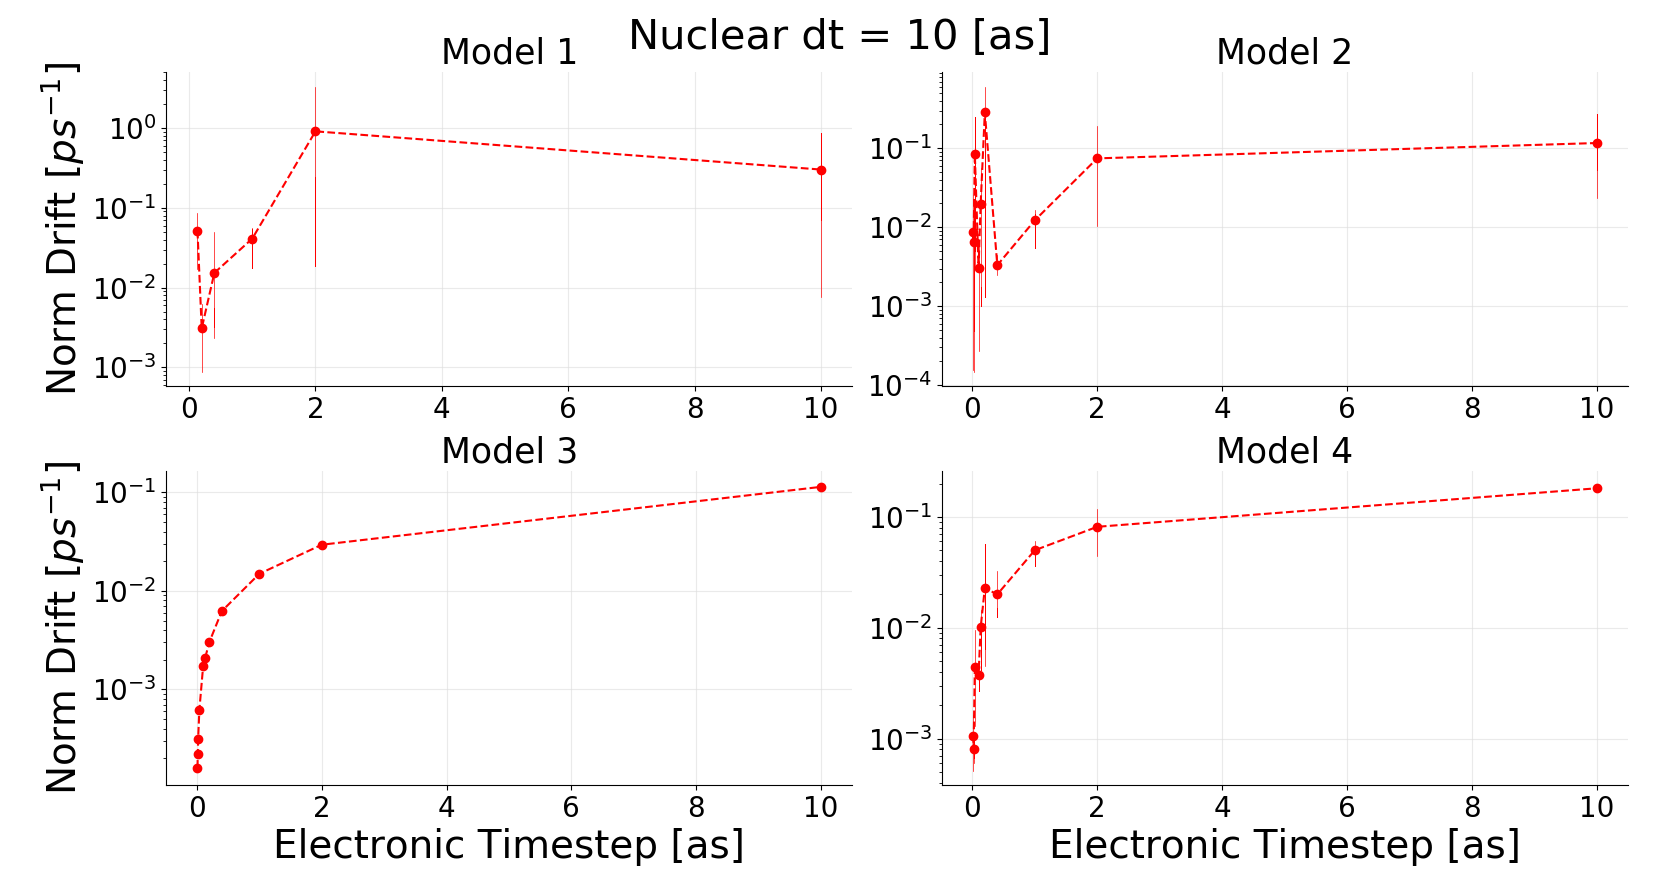
\includegraphics[width=\textwidth]{/home/matt/Documents/PhD/PhD_Thesis/img/CTMQC/TullyModels/CTMQC_Norm_Conservation.png}
	\caption{\label{fig:CTMQCNormCons}The norm conservation when using standard CTMQC as outlined in the literature for each of the Tully models. These simulations were ran with a high initial momentum. The red markers show data points and vertical bars show error bars associated with each point.}
\end{figure}
\\\\
The calculation of the quantum momentum is discussed in detail in Min, 17 \cite{min_ab_2017} and outlined in the introduction to the thesis in section \ref{sect:QM_Calc}. As mentioned in that section, the denominator in the expression for $\mathbf{R}_{lk, \nu}$ may be positive or negative and when it switches between each it can approach zero very closely. If this denominator approaches zero more quickly that the numerator then we can see large divergence in the $\mathbf{R}_{lk, \nu}$ term which can lead to large norm drifts. This is highlighted in figure \ref{fig:QlkSpike}.

\subsubsection{Quantum Momentum Instabilities}
\label{sect:QlkSpikes}
\begin{figure}[ht]
	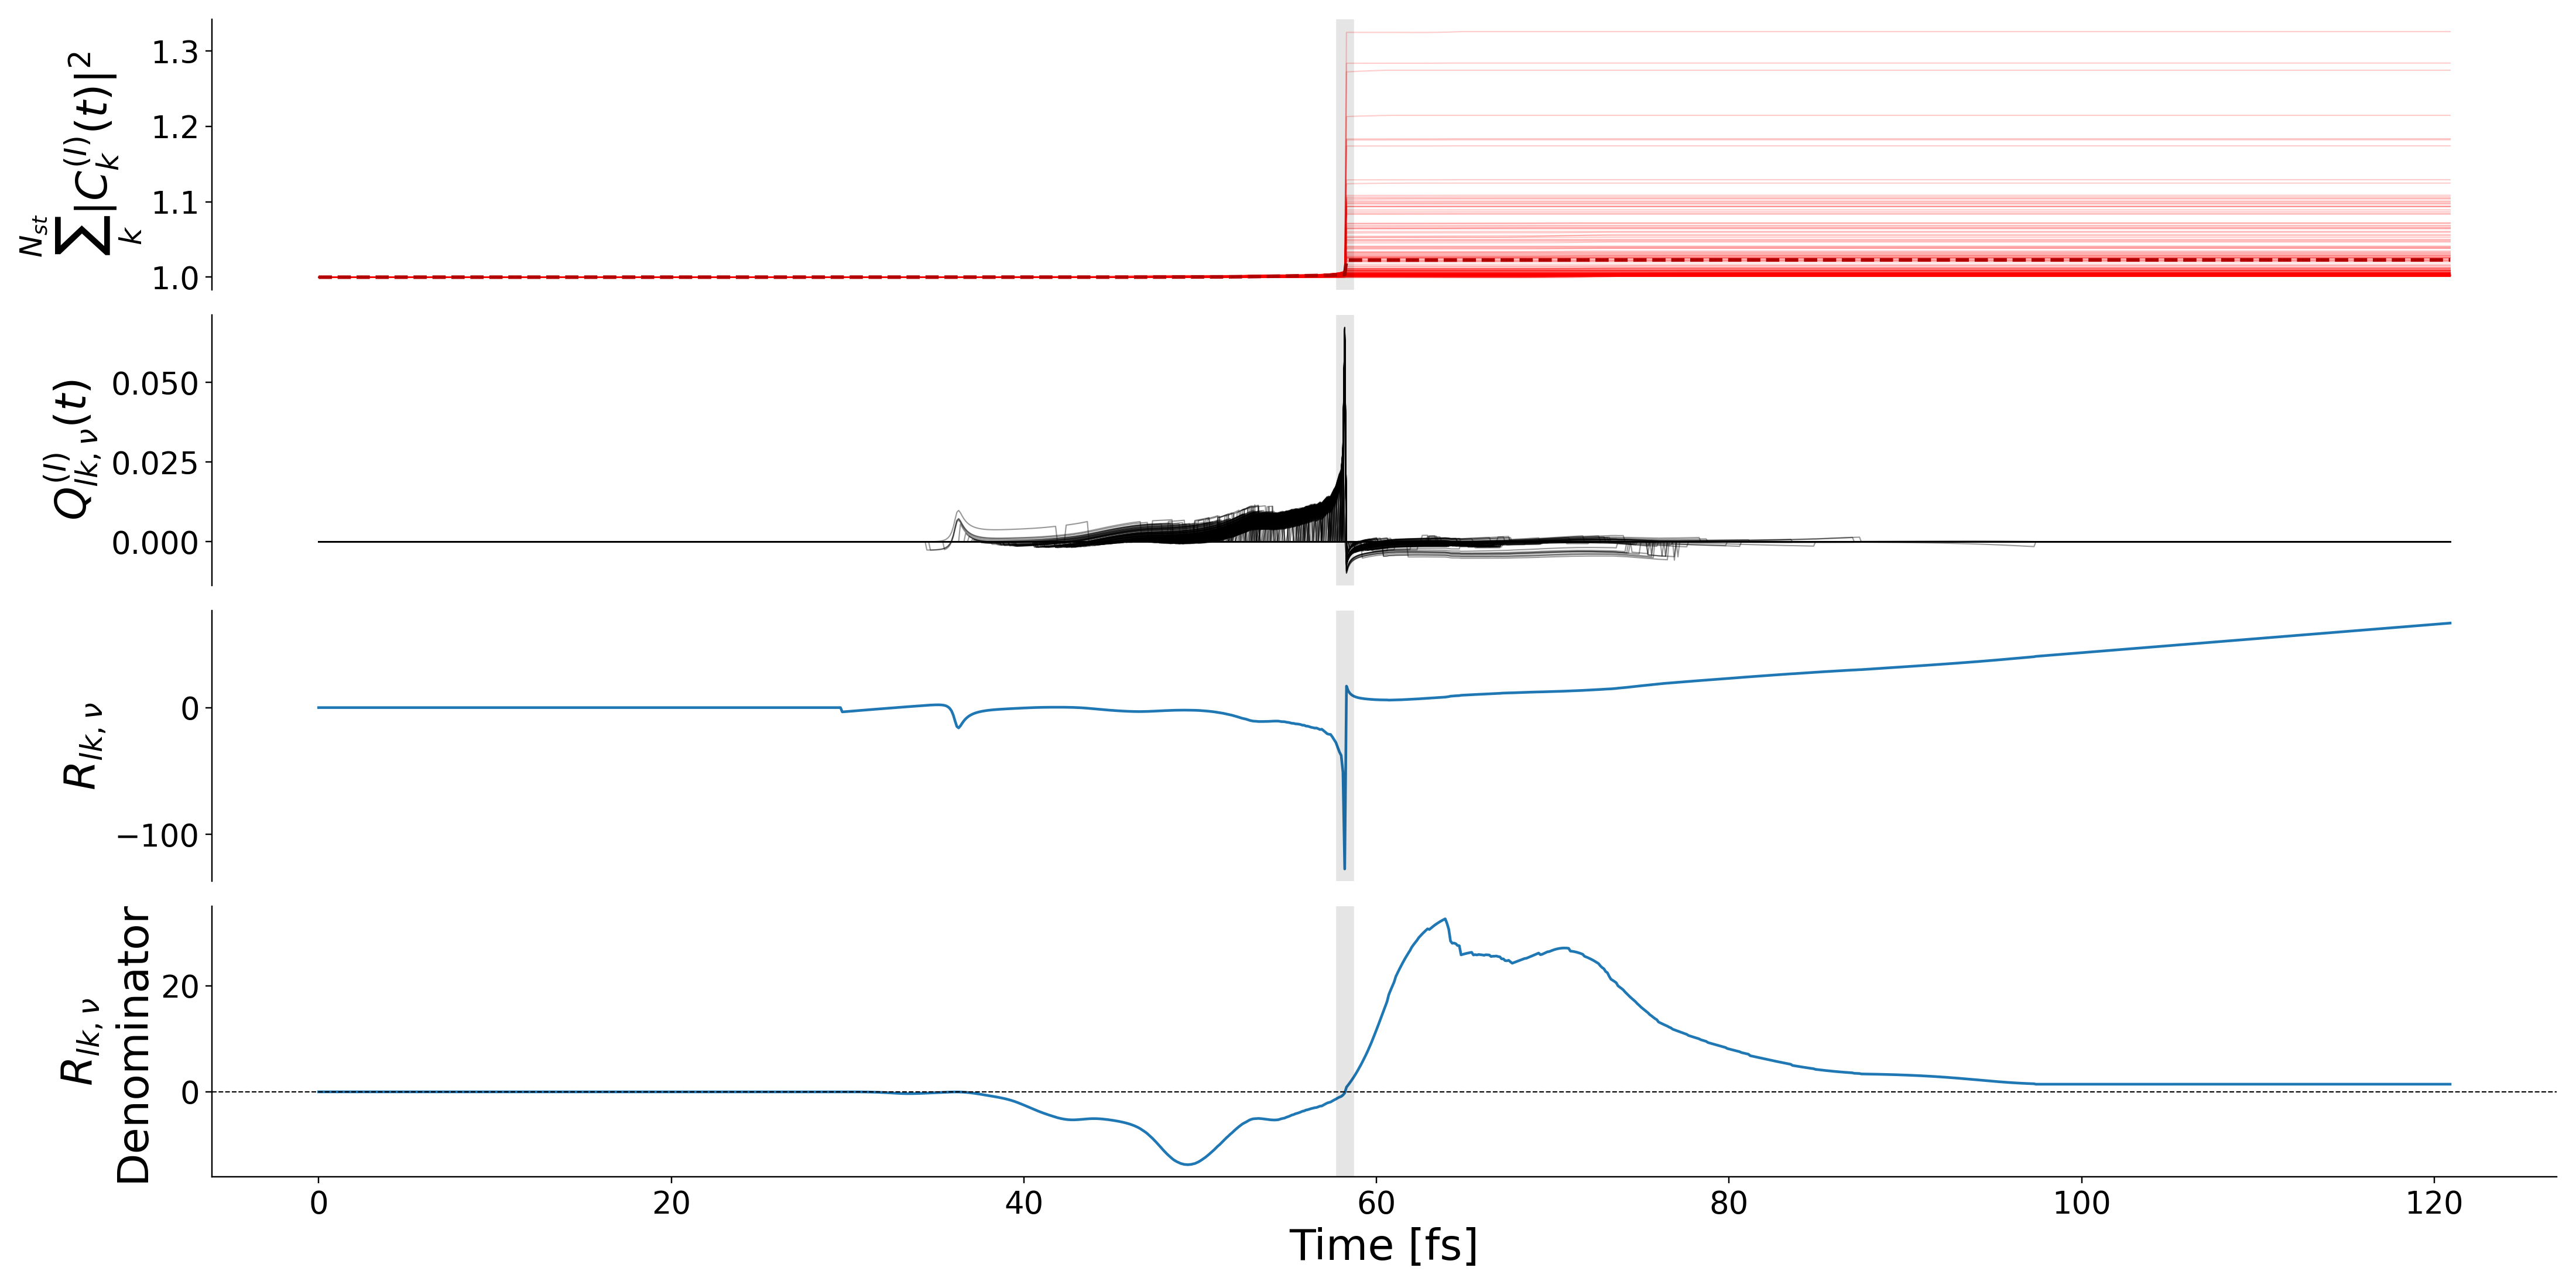
\includegraphics[width=\textwidth]{./img/CTMQC/TullyModels/Spikes/RlkDenom_Rlk_Qlk_Norm.png}
	\caption{\label{fig:QlkSpike}As the denominator of the $\mathbf{R}_{lk,\nu}$ term approaches zero (bottom panel) the full $\mathbf{R}_{lk, \nu}$ term (2$^{\text{nd}}$ to bottom panel) can approach infinity which propagates through the $\mathcal{Q}_{lk, \nu}^{(I)}$ term (2$^{\text{nd}}$ to top panel) causing discontinuities and norm drift in the populations (top panel). The grey vertical bar denotes the region the denominator approaches 0. The thin solid red lines in the top panel show the norm drift for individual replicas.}
\end{figure}
\noindent In figure \ref{fig:QlkSpike}, as the denominator of quantum momentum intercept (the bottom panel) approaches 0 the $\mathbf{R}_{lk, \nu}$ term may spike causing a discontinuity in the populations (through the quantum momentum). The reason this only occurs in Models 1, 2 and 4 is due to the fact that the difference in the adiabatic momenta terms ($\mathbf{f}_{l, \nu}^{(I)} - \mathbf{f}_{k, \nu}^{(I)}$) doesn't cross 0 in Model 3 as the time-derivative of the adiabatic energies is always either positive or negative. 
\\\\
In order to correct for this divergence I have investigated a number of alterations to the calculation of the quantum momentum. These depend on the detection of the spikes/divergences in the $\mathbf{R}_{lk, \nu}$ term and then the appropriate treatment of them. A divergence is recorded is 2 conditions are met. First is a simple threshold on the time-derivative of the intercept term, i.e. $|\frac{\delta}{\delta t} \mathbf{R}_{lk, \nu}| > thresh$. The second condition is a threshold on the intercept denominator i.e. $|\mathbf{R}denom_{lk, \nu}| < thresh$. For example, if the absolute time-derivative of the $\mathbf{R}{lk, \nu}$ term is larger than a value (say 5) and the bottom of the fraction in equation \eqref{eq:Rlk} is within 0.01 of 0 then we assume the $\mathbf{R}_{lk, \nu}$ term is diverging and the simulation code then uses a different method of propagating the electronic coefficients.
\noindent The alternative propagation methods that have been investigated are:
\begin{enumerate}
	\item Use Ehrenfest Dynamics (set e.g. $\mathcal{Q}_{lk, \nu}$ term to 0).
	\item Extrapolate the value of $\mathbf{R}_{lk, \nu}$ from values before the divergence (see appendix \ref{ap:RlkExtrap}).
	\item Switch to using the alternative intercept $\mathbf{R}_{0, \nu}^{(I)}$ (see appendix \ref{ap:AltIntercept}).
\end{enumerate}
of these 3 methods, method 3 was the most successful in reducing the norm drift in the Tully Models as can be seen in figure \ref{fig:NormConsCorr}.
\begin{figure}[ht]
	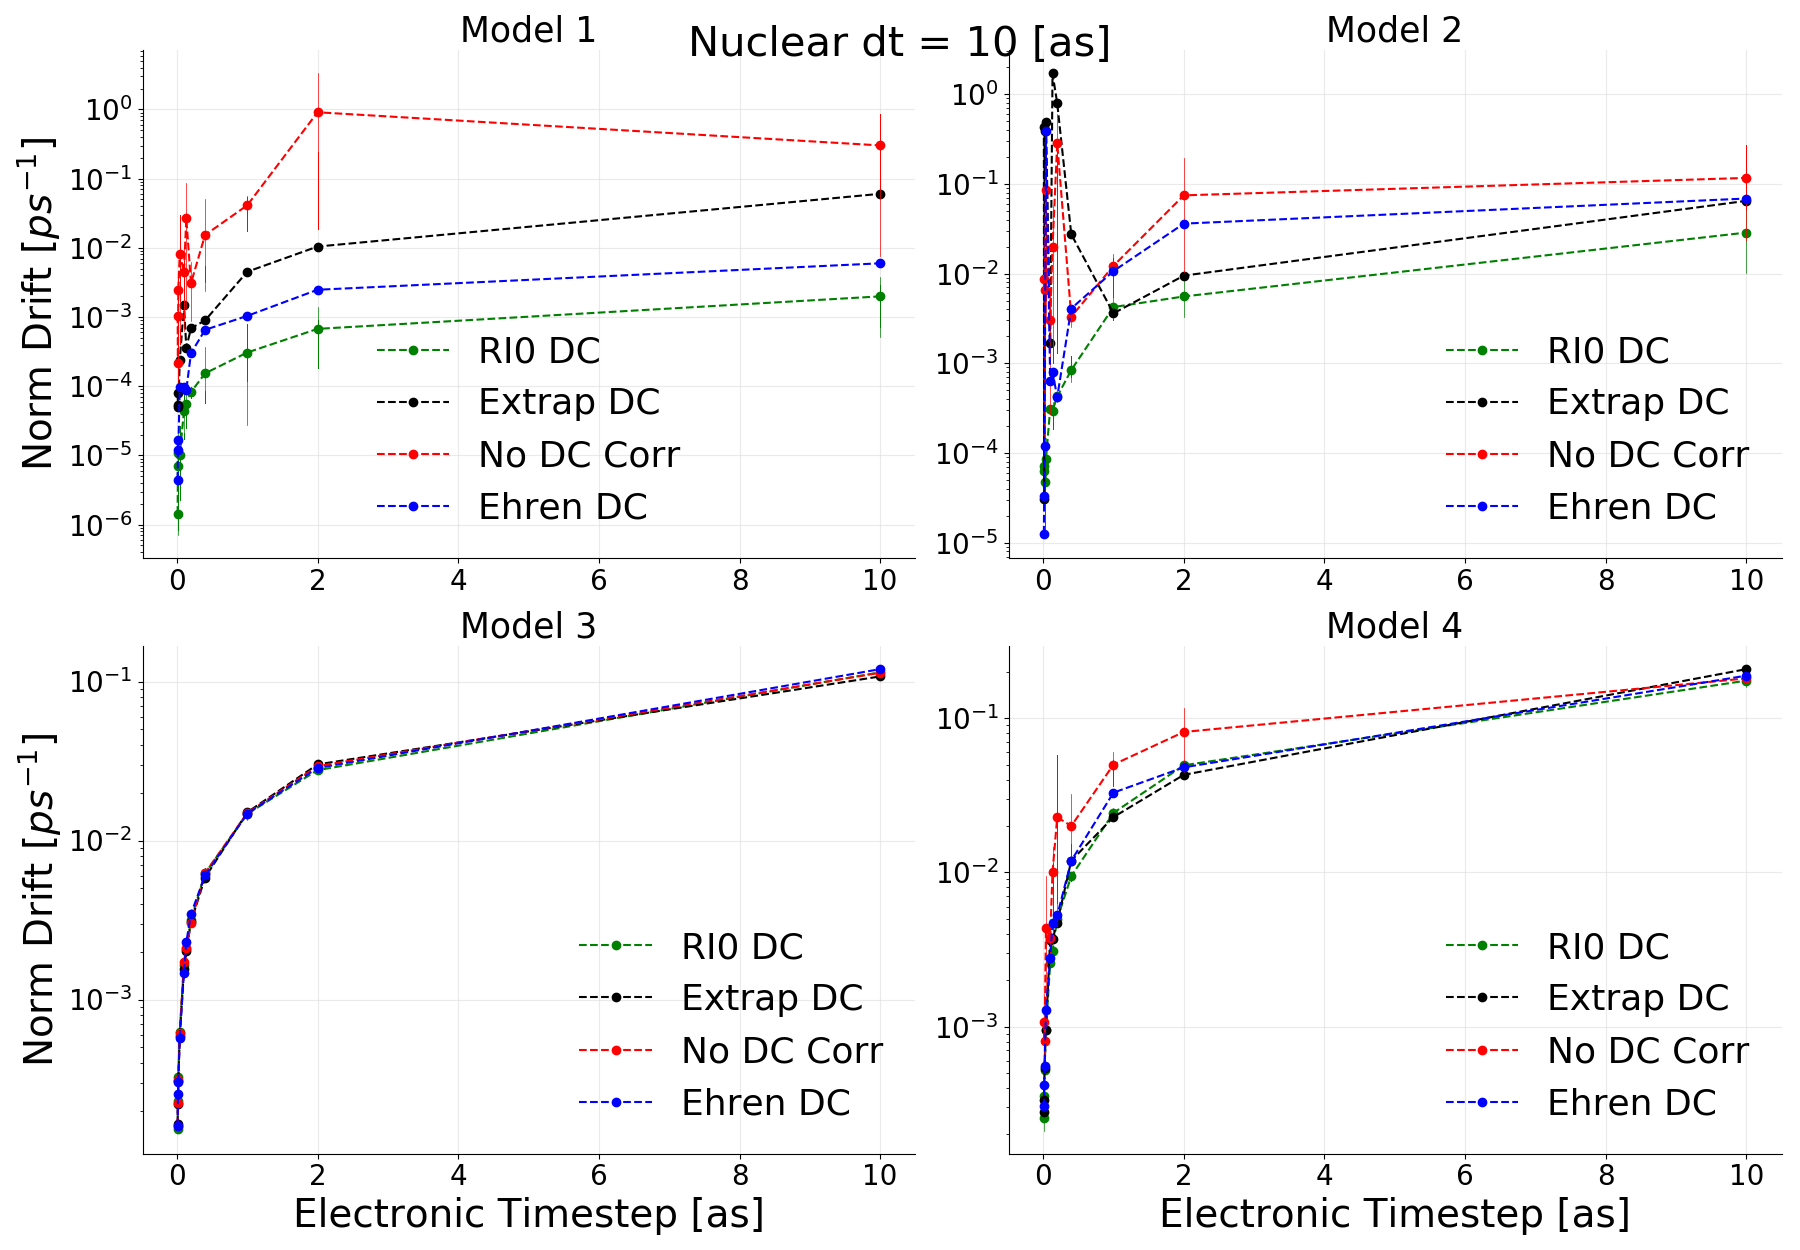
\includegraphics[width=\textwidth]{img/CTMQC/TullyModels/CTMQC_Norm_Conservation_wCorr.png}
	\caption{\label{fig:NormConsCorr}Norm conservation in CTMQC after applying a divergence correction to the $\mathbf{R}_{lk, \nu}$ term. RI0 refers to method 3, Extrap DC refers to method 2 and Ehren DC refers to method 1. No DC Corr shows the population norm without any corrections applied.}
\end{figure}
\\
In figure \ref{fig:NormConsCorr} we see the norm drift results after the 3 $\mathbf{R}_{lk, \nu}$ correction methods have been applied. The red curve shows the original data (as in figure \ref{fig:CTMQCNormCons}) with its large divergences in the norm drift. The green curve shows the alternative intercept method, the blue curve shows the effect of switching to Ehrenfest during the $\mathcal{Q}_{lk, \nu}^{(I)}$ spikes and the black shows a method that involved extrapolating the $\mathbf{R}_{lk, \nu}$ value from data before the spike began. We can see clearly all 3 methods improve the norm drift, though using the alternative intercept seems to help the most. Model 3 is not affected as we do not see these divergences in the $\mathbf{R}_{lk, \nu}$ due to the denominator in this particular model never crossing from positive to negative (through zero). It is important to note that in each of the models with the divergence correction applied all models exhibit the expected trend of decreasing the time-step improves norm conservation. However, the norm conservation in all 4 models is still significantly higher ($\sim$ 7-8 orders of magnitude) higher than that of Ehrenfest.  This is due to the product of the adiabatic populations, $|C_{l}^{(I)}|^2 |C_{k}^{(I)}|^2$, being used in the calculation of the quantum momentum. These can be a more quickly varying quantity than just the adiabatic populations alone -thus require a smaller timestep to adequately sample in a continuous way.

\subsection{Mathematical Tests}
Multiple tests of the implementation of the quantities in the equations have been implemented in the code to ensure correct outputs. A checklist of any mathematical tests is given below:
\begin{itemize}
  \item Checking the (anti-)symmetry of the (NACV) Hamiltonian when constructed
  
  \item Comparing the adiabatic momentum term to post-production time-integrated adiabatic energies (using trapezium rule \cite{NumericalAnalysis})
  
  \item Checking special case solutions when all replicas are initialised at the same position such as:
	\begin{itemize}
	  \item $\mathcal{Q}_{lk, \nu}^{(I)} = 0$
	  \item CTMQC = Ehrenfest
	\end{itemize}

  \item Checking special cases for when $\sigma$ is replica independent (i.e. $\sigma^{(I)} = \sigma$):
	\begin{itemize}
	  \item $\sigma = \frac{\hbar}{2 \sigma^2}$
	  \item $\mathbf{R}_{lk, \nu} = \mathbf{R}_{\nu}^{(I)} \frac{\hbar}{2 \sigma^2}$ (Assuming the positions, $\mathbf{R}_{\nu}^{(I)}$ are also replica independent)
	\end{itemize}

  \item If all adiabatic population is localised on a single state ($|C_{l}^{(I)}|^2 = [1, 0, 0, \cdots, 0]$). Then we get Ehrenfest dynamics on that replica.
  \item Solving the static Schr\"odinger equation gives Rabi oscillation \cite{FeynmanLectVol3}. See appendix \ref{ap:Rabi}.
\end{itemize}

I have also provided 2 (more substantial) mathematical tests for the code below in the following sections.
\subsubsection{Time Derivative of Replica-Sum of Adiabatic Populations}
\begin{figure}[ht]
	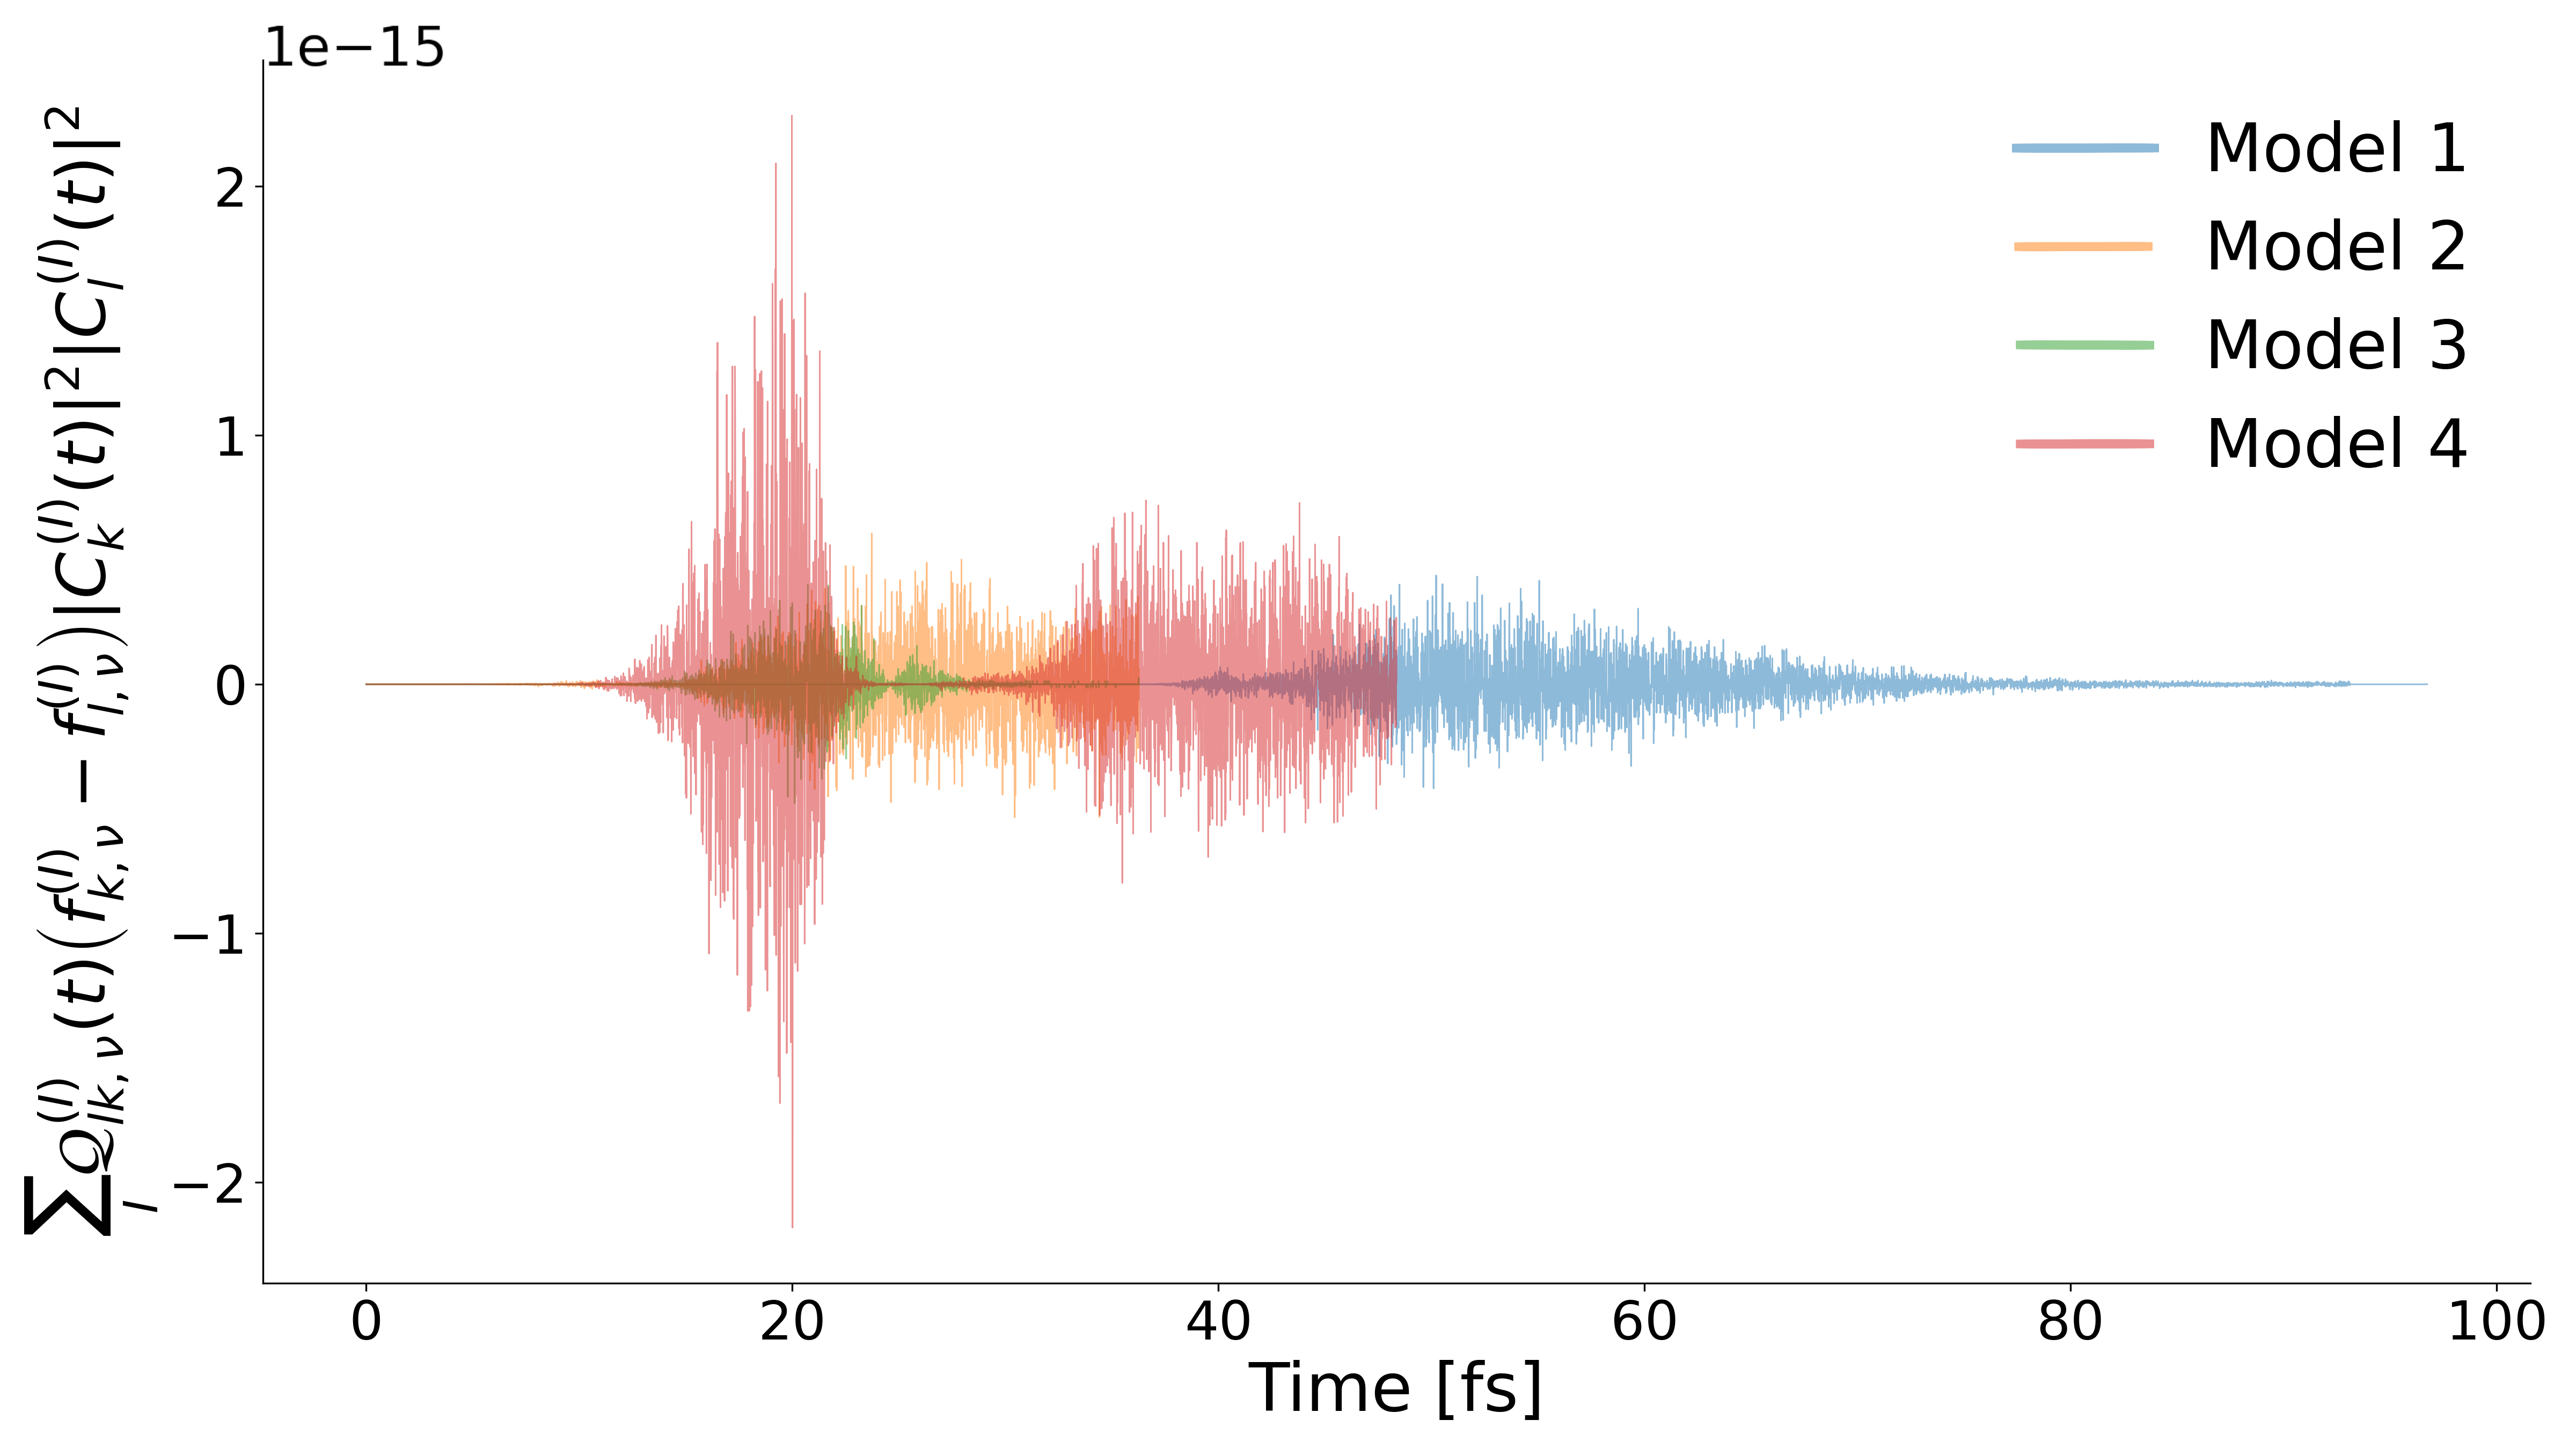
\includegraphics[width=\textwidth]{./img/CTMQC/TullyModels/CTMQC_S27.png}
	\caption{\label{fig:S27}The conserved quantity given in equation \eqref{eq:S27} (y-axis). Each color represents data outputted by a simulation using a different model (specified in the legend). Each time-series is plotted with a translucent color meaning each model's data can be seen at once.}
\end{figure}

\noindent In the SI of Min, 17 \cite{min_ab_2017} a conservation equation (S27) is given. This is repeated below in equation \eqref{eq:S27}
\begin{equation}
	\sum_{I} \mathcal{Q}_{lk, \nu}^{(I)}(t) \left( f_{k, \nu}^{(I)} - f_{l, \nu}^{(I)} \right) |C_{k}^{(I)} (t)|^2 |C_{l}^{(I)} (t)|^2 = 0  \qquad \forall l, k, \nu
	\label{eq:S27}
\end{equation}

An example time-series of this quantity is given in figure \ref{fig:S27} for each Tully model. The data used to calculate come from simulations of each of the Tully models using the parameters given in appendix \ref{ap:tully_params}. No smoothing was used for the $\mathbf{R}_{lk, \nu}^{(I)}$ term. It can be seen in this figure that the conservation quantity hovers around 0 for each model with a maximum deviation of 10$^{-15}$ m$_{e}$Ha.

\subsubsection{Numerical Check of the Propagation Matrix}
\label{sect:sumXqmll}
As the equations are currently formulated another numerical test validating the quantum momentum part of the propagation equations for the coefficients can be used. The CTMQC equation for the propagation of the adiabatic expansion coefficients is given in equation \eqref{eq:elec_adiab}. The quantum momentum part of this equation is given below in equation \eqref{eq:qmCTMQCAdiab}. 
\begin{equation}
  \mathbb{X}_{qm, ll}^{(I)} = \sum_{\nu=1}^{N_n}\sum_{k} \frac{\mathcal{Q}_{lk, \nu}^{(I)}}{\hbar     M_\nu} \cdot \left[ \mathbf{f}_{k,\nu}^{(I)} - \mathbf{f}_{l,\nu}^{(I)}   \right] |C_{k}^{(I)}|^2
  \label{eq:qmCTMQCAdiab}
\end{equation}
Where $\mathbb{X}_{qm, ll}^{(I)}$ is the diagonal matrix that, when multiplied with the adiabatic expansion coefficients, gives the quantum momentum contribution to the propagation of the expansion coefficients.
\\\\
We can test the construction of this matrix within the code by multiplying by the adiabatic populations and summing as shown in equation \eqref{eq:NumericalTestXqmll}. It can be shown, assuming perfect norm conservation, that this should equal exactly 0 -due to the symmetry of the $|C_{l}^{(I)}|^2|C_{k}^{(I)}|^2$ and the quantum momentum matrix. This is checked for every timestep during propagation.

\begin{equation}
  \sum_{l} \mathbb{X}_{qm, ll}^{(I)} |C_{l}^{(I)}|^2 = 0
  \label{eq:NumericalTestXqmll}
\end{equation}


\subsection{Energy Conservation}
In Agostini \cite{agostini_quantum-classical_2016} it is stated that the approximate potential energy is given by the same equation as in Ehrenfest, i.e. equation \eqref{eq:EhrenfestEnergyConservation} a population weighted average of the potential energy surfaces. The 4 high momentum Tully models were simulated with various nuclear timesteps and a straight line of best fit was fitted to the total energy term.
\begin{figure}[ht]
  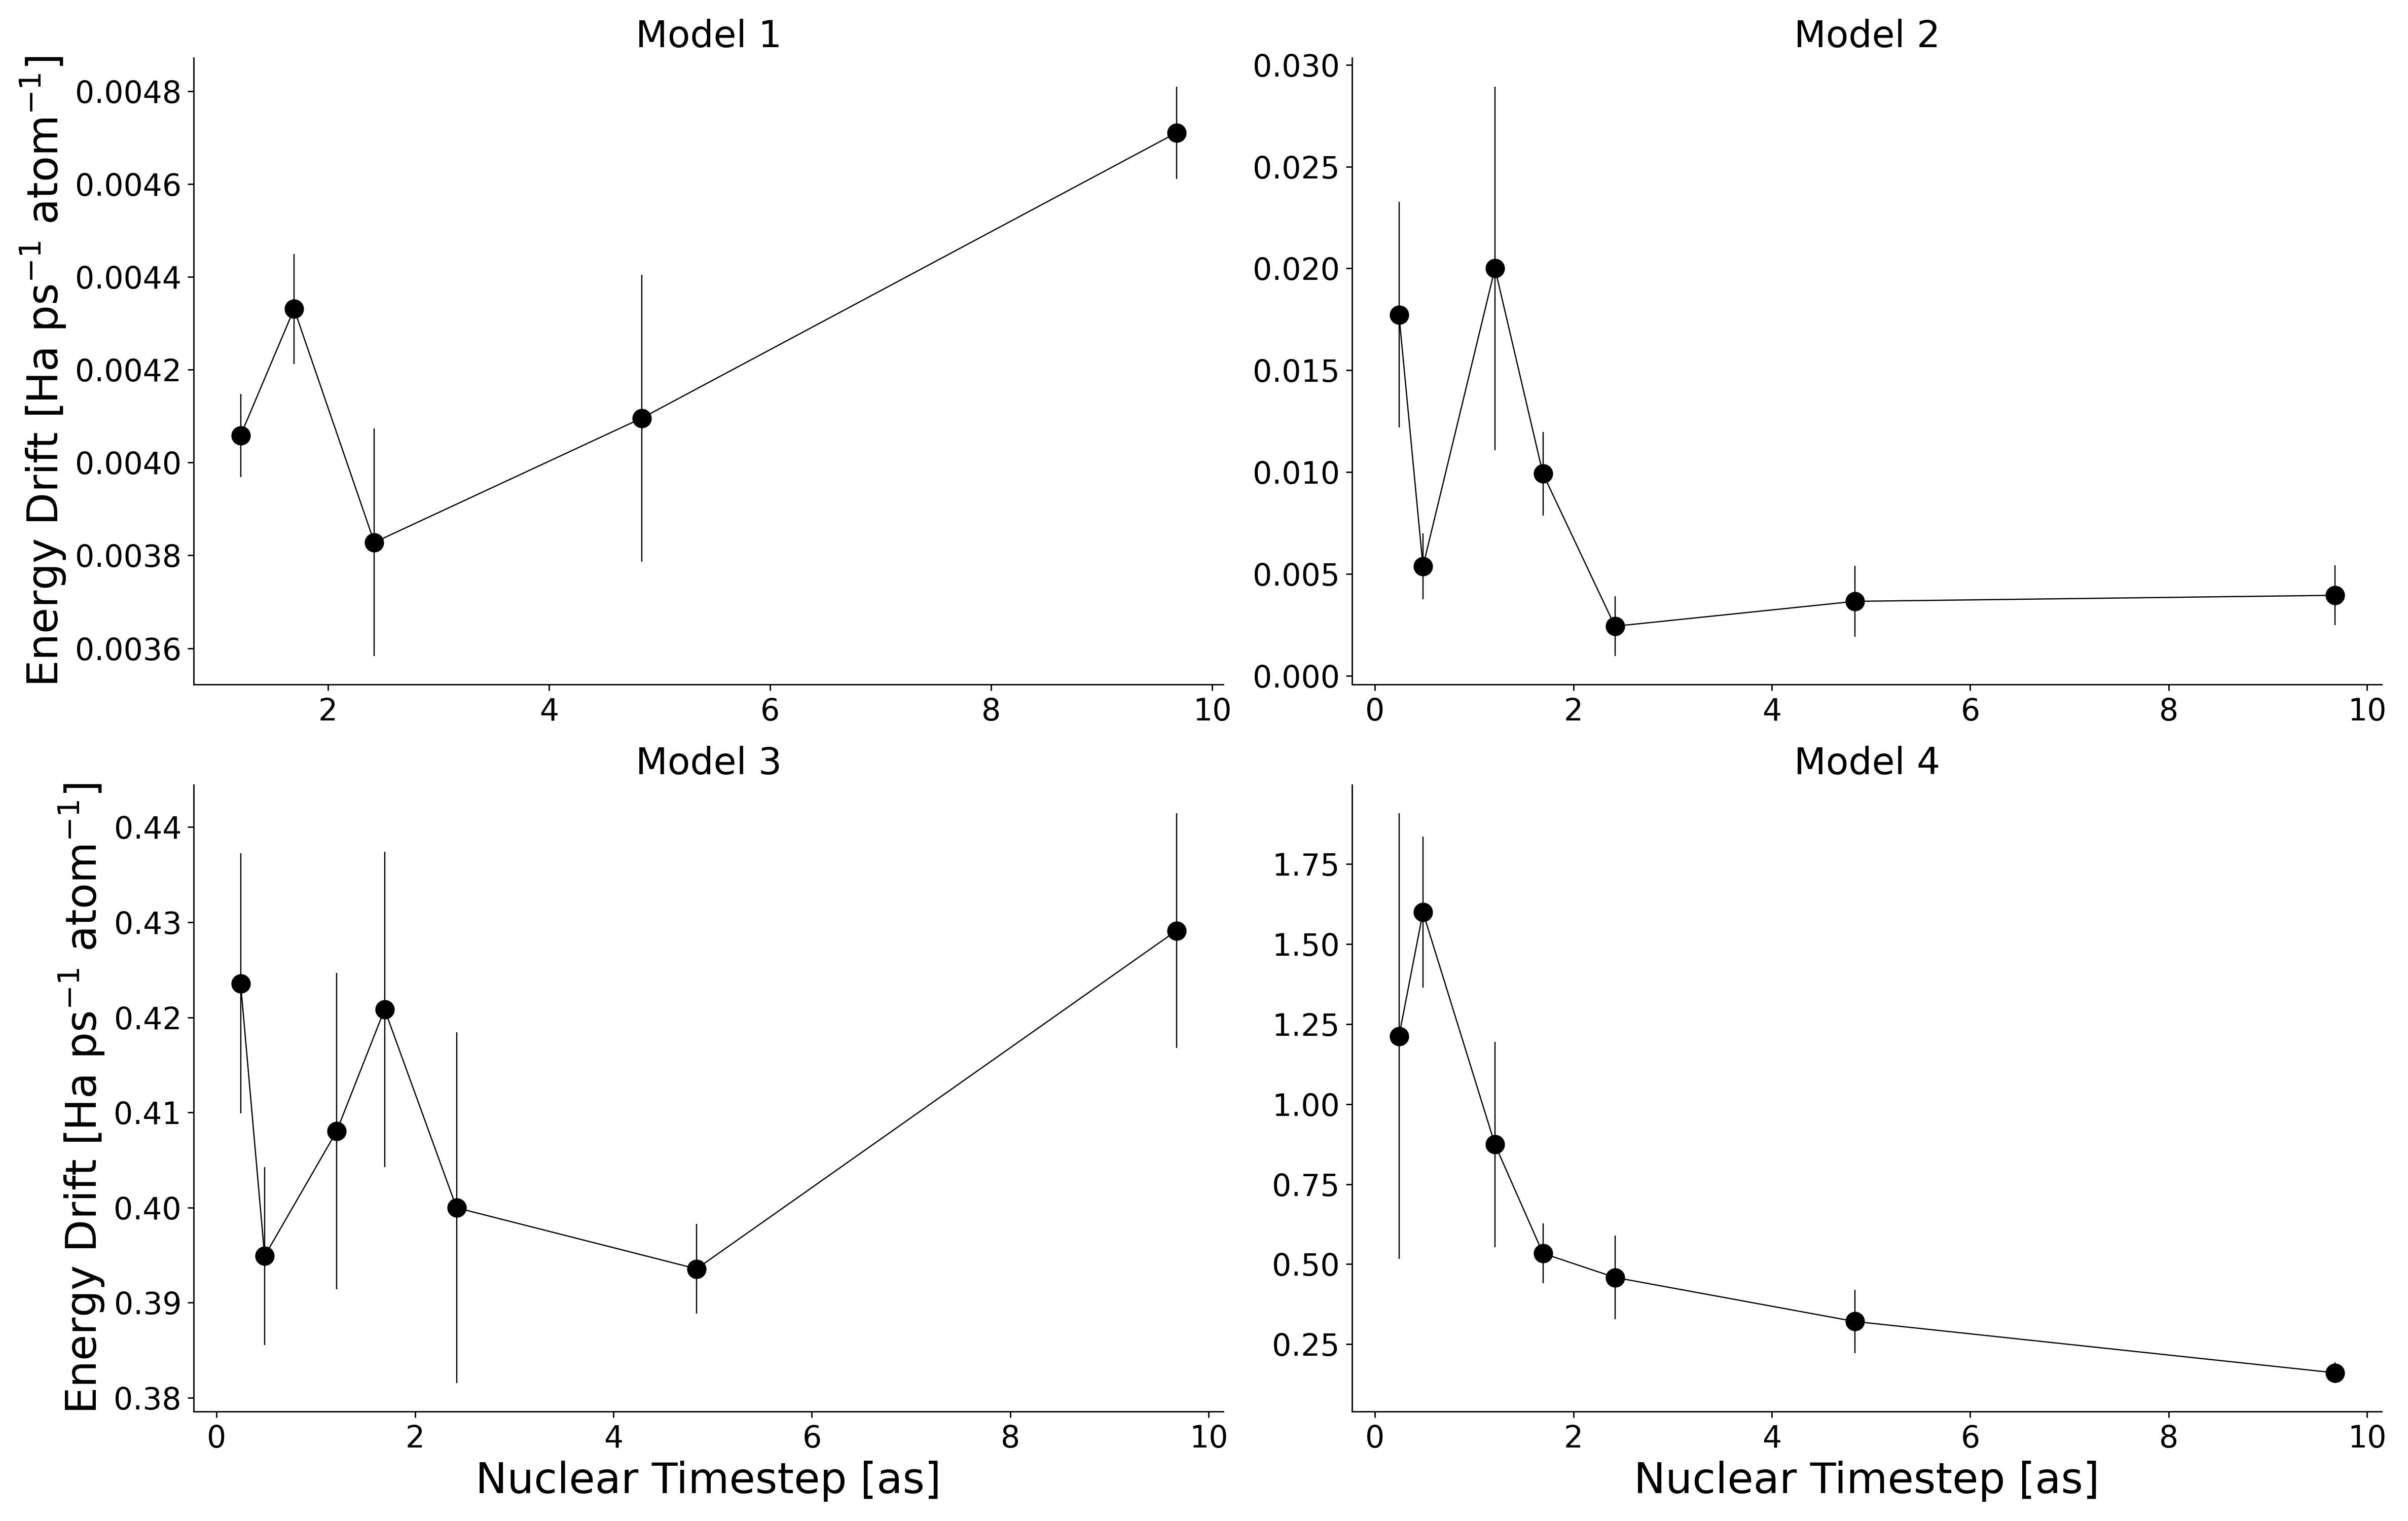
\includegraphics[width=\textwidth]{./img/CTMQC/TullyModels/CTMQC_EnerCons.png}
  \caption{\label{fig:CTMQC_EnergyCons}Energy drift in the 4 Tully models using the full CTMQC equations. Error bars are from multiple simulations carried out with different random sampling of the initial positions and momenta.}
\end{figure}
\\
As can be seen in figure \ref{fig:CTMQC_EnergyCons} the energy conservation in CTMQC does not improve with a decreasing nuclear timestep. In fact in the energy conservation worsens with decrease nuclear timestep in some models such as model 4. Additionally, in models 2 and 4 the errorbar increases as the timestep decreases. This is caused by an increased likelihood of coming across a divergence in the quantum momentum that can't be properly corrected, due to more steps being simulated. In model 3, the error bar stays the fairly consistent, and the energy conservation doesn't change with respect to the timestep. In this model there are no quantum momentum divergences which means the poor energy conservation is caused by something else. The potential energy as given in Agostini \cite{agostini_quantum-classical_2016} is an approximation and to achieve energy conservation comparable to Ehrenfest this may need amending.

\subsection{Comparisons to literature}
\begin{figure}[ht]
	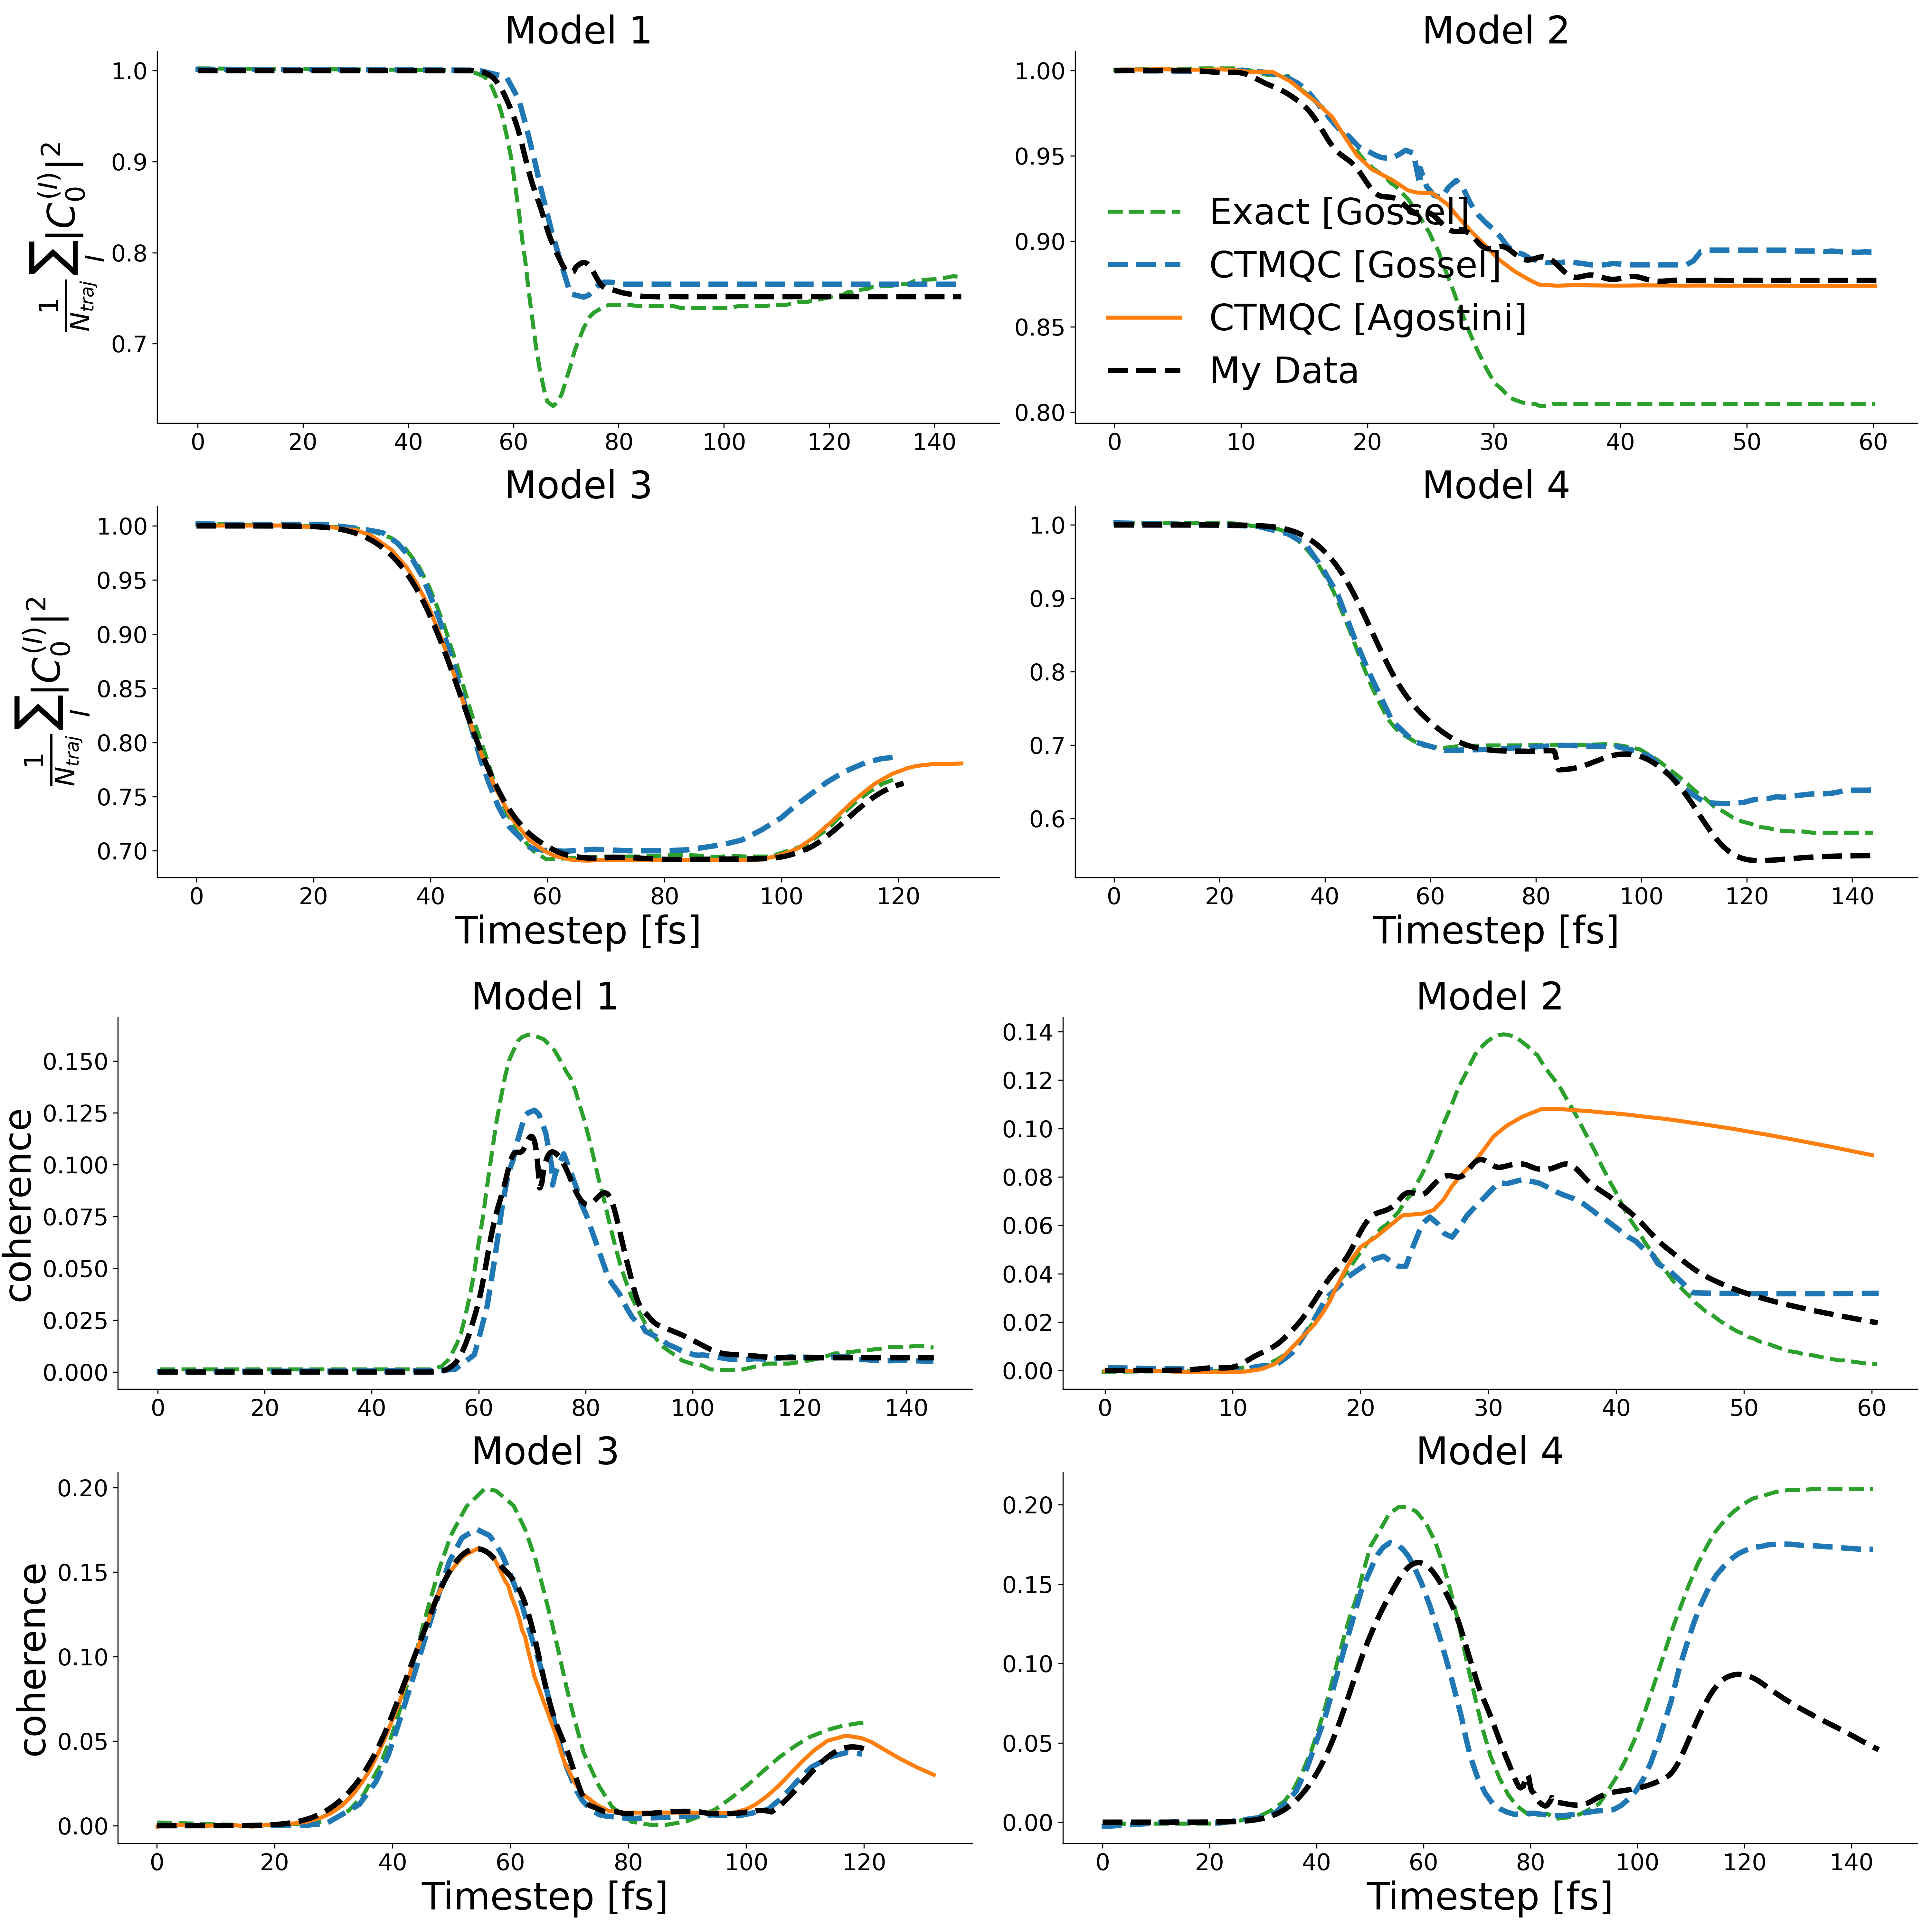
\includegraphics[width=\textwidth]{img/CTMQC/TullyModels/CTMQC_lowMom.png}
	\caption{\label{fig:LitCompCTMQCTullyLow}A comparison of my implementation of full CTMQC (for 4 model Hamiltonians) and results from the literature for the low momentum cases. The black dashed lines show my CTMQC data (ground state ad pops), the orange dashed lines are data from Agostini \cite{agostini_quantum-classical_2016} and the blue solid lines are from Gossel \cite{gossel_coupled-trajectory_2018}. The solid green line shows data from exact quantum mechanical simulations given in Gossel. The figures are labelled with their model number, whether the initial momentum was high or low and whether the populations or coherence indicator was plotted.}
\end{figure}
\begin{figure}[ht]
	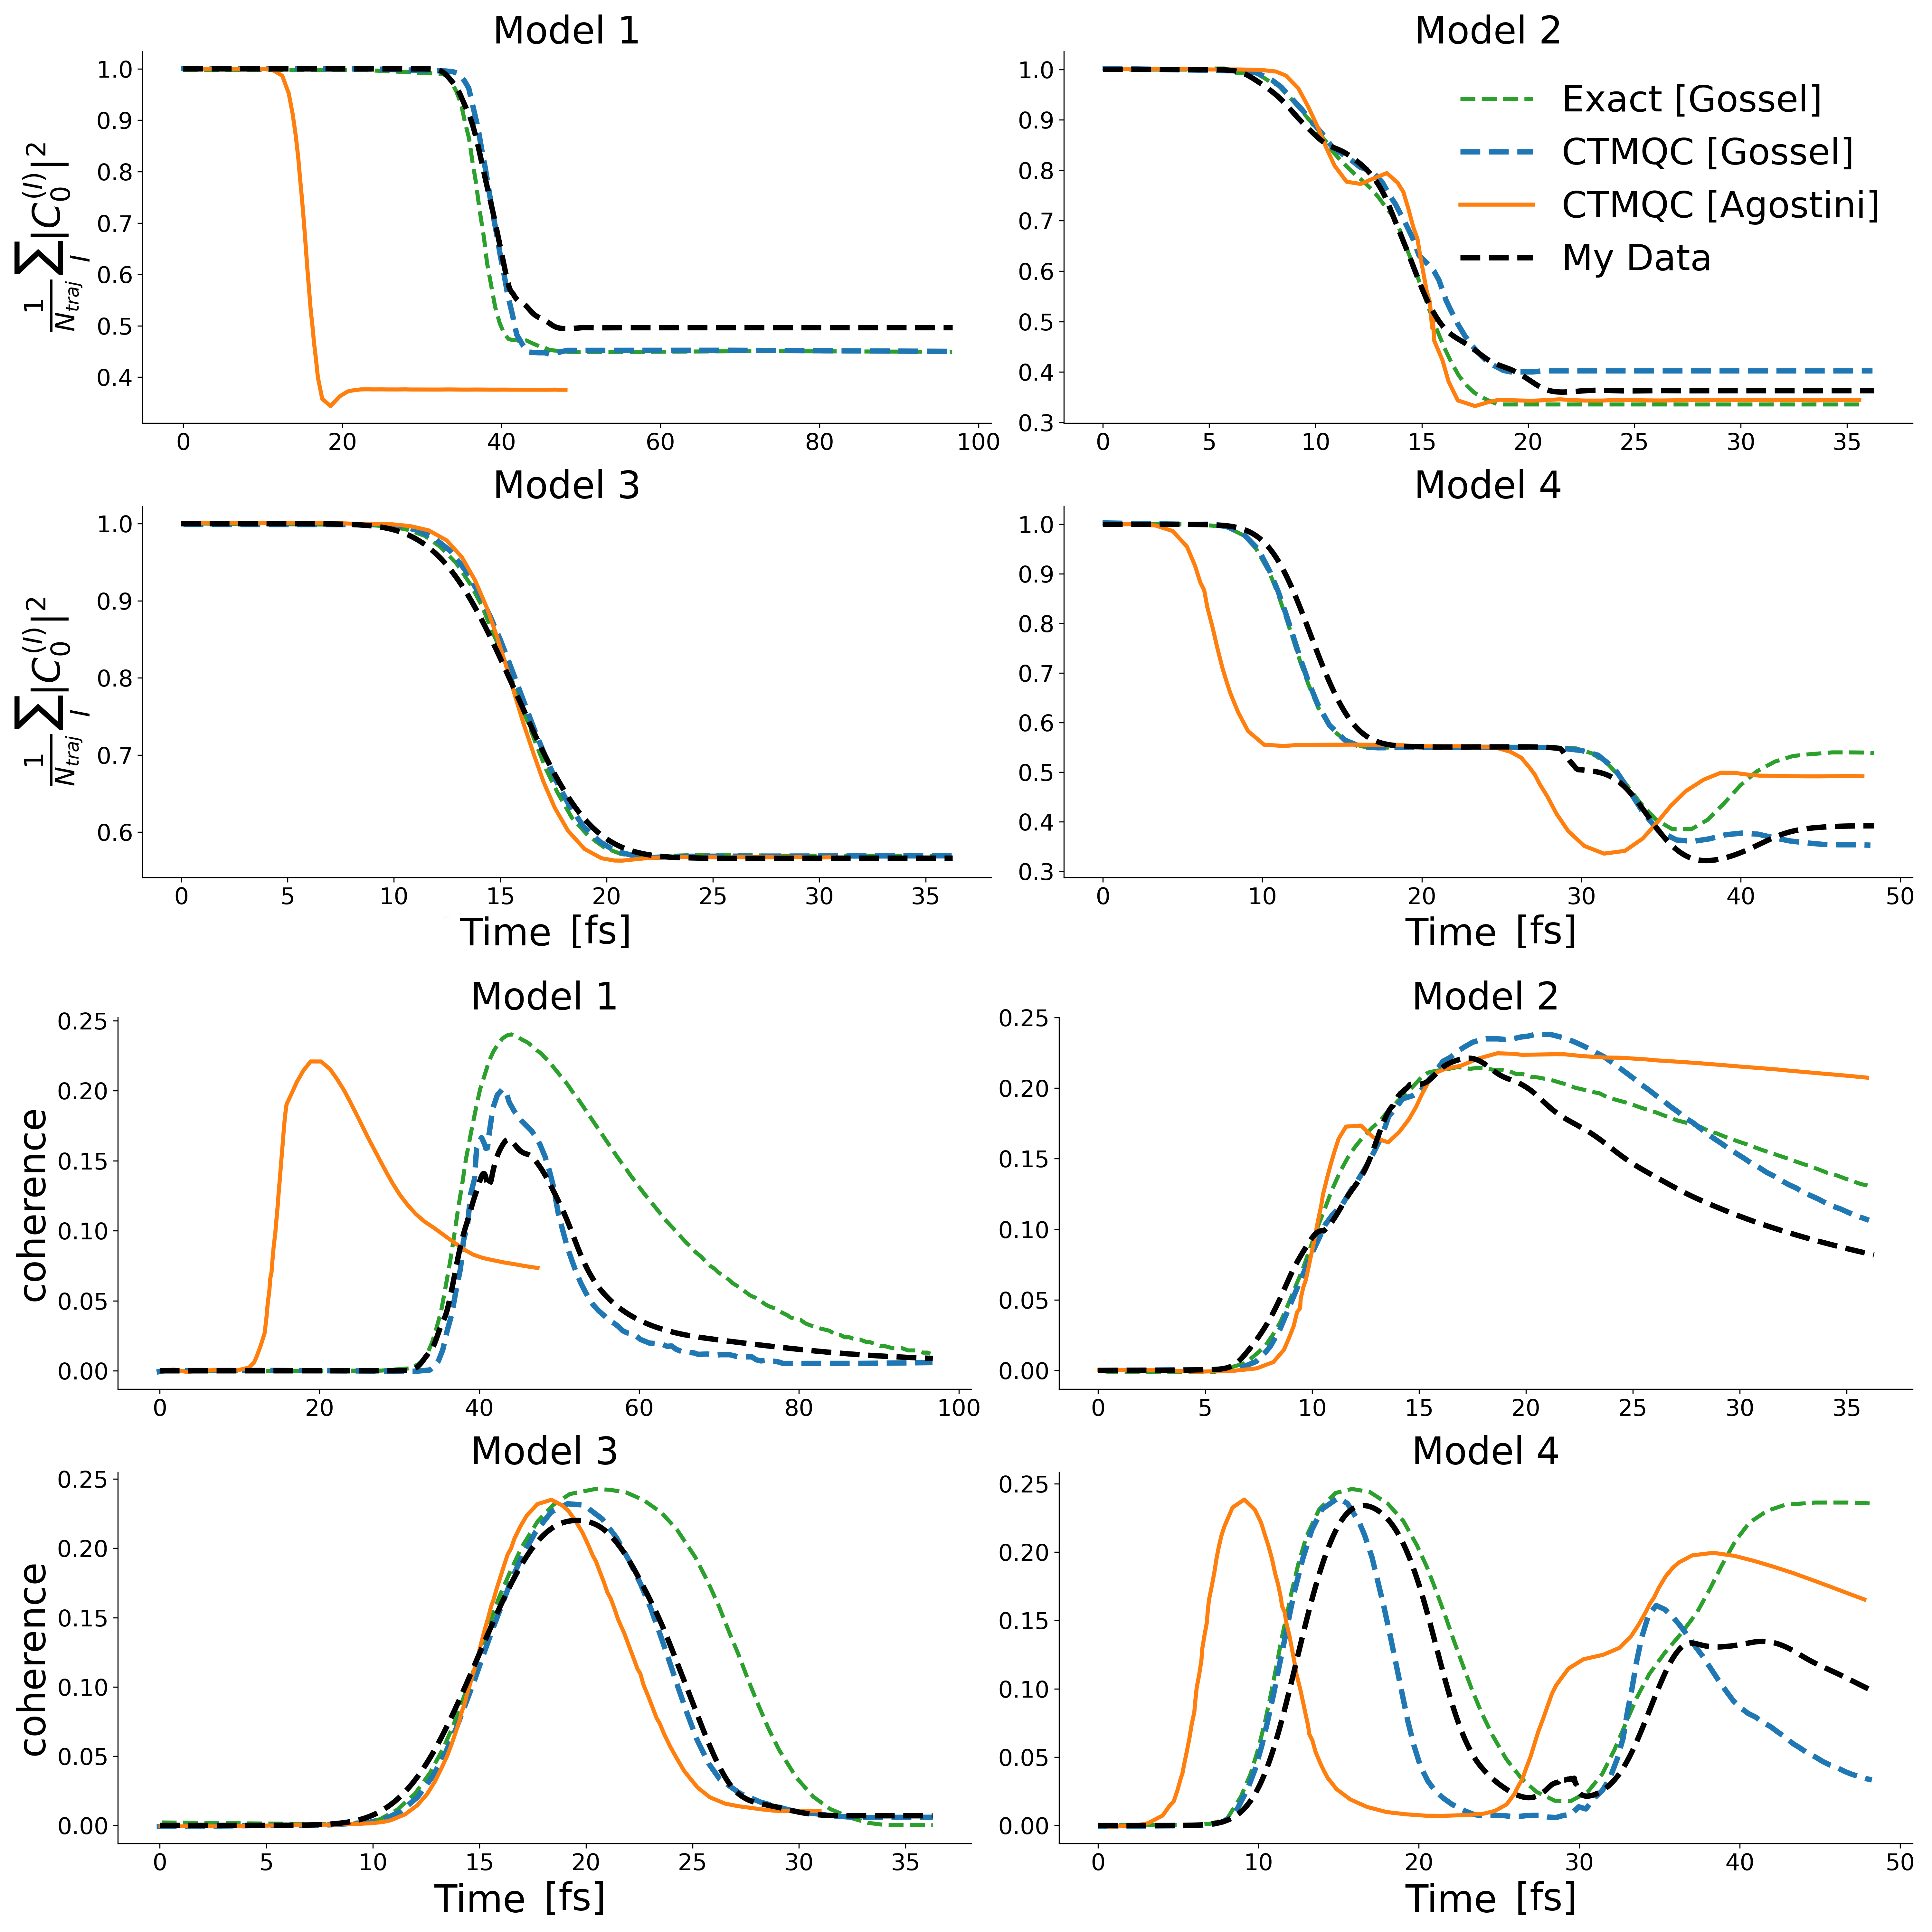
\includegraphics[width=\textwidth]{img/CTMQC/TullyModels/CTMQC_highMom.png}
	\caption{\label{fig:LitCompCTMQCTullyHigh}A comparison of my implementation of full CTMQC (for 4 model Hamiltonians) and results from the literature for the high momentum cases. The black dashed lines show my CTMQC data (ground state ad pops), the orange dashed lines are data from Agostini \cite{agostini_quantum-classical_2016} and the blue solid lines are from Gossel \cite{gossel_coupled-trajectory_2018}. The solid green line shows data from exact quantum mechanical simulations given in Gossel. The figures are labelled with their model number, whether the initial momentum was high or low and whether the populations or coherence indicator was plotted.}
\end{figure}

As in section \ref{sect:EhrenCompare} we can compare the CTMQC results to those published before in Gossel \cite{gossel_coupled-trajectory_2018} and Agostini \cite{agostini_quantum-classical_2016}. These results are given in figures \ref{fig:LitCompCTMQCTullyLow} and \ref{fig:LitCompCTMQCTullyHigh}. This time, unlike in the Ehrenfest code, we see some discrepancies between the 3 results which cannot solely be explained as small errors from different sampling of initial positions or from errors in extracting data from graphs in the papers. We can see that the errors mainly appear in the coherence indicator, looking at the bottom row in figures \ref{fig:LitCompCTMQCTullyLow} and \ref{fig:LitCompEhrenTullyHigh} it appears that both the Agostini and Gossel results match mine (dashed black line) very closely. The largest difference is seen in model 4, high momentum where the Gossel data and mine follow a similar trend and the Agostini data follows the exact curve more closely. The reason for this is a difference in the way the adiabatic momenta terms are handled. In the Gossel paper,  a method to reset the adiabatic momenta to 0 for each replica when the adiabatic populations collapse onto a pure adiabatic state (within a tolerance) is used. If this resetting is turned off then the populations in model 4 follow the Agostini results exactly. While resetting the adiabatic momenta worsens the calculation of the adiabatic populations in the model 4 simulations, it improves the convergence of the coherence indicator in the model 2 simulations. I will show later how using a method to dynamically alter the gaussian width parameter, used to calculate the quantum momentum, can improve the model 4 results markedly. Other deviations in results for the populations are due to a slightly different sampling of initial positions, a different handling of divergences in the quantum momentum term and constructing the $\mathcal{Q}_{lk, \nu}^{(I)}$ term with a different width parameter ($\sigma$) -which isn't specified in each of the paper the results have been taken from. The differences in my results and those given in the literature are on the same scale as the differences already presented in the literature and they are not large enough to invalidate my implementation. The discrepancies present between the results in the papers presented here are probably caused by the same small algorithmic differences causing minor discrepancies in my results. The fact many of the literature results agree exactly with my implementation can be taken as a confirmation that my implementation is working well. 

\section{Construction of the quantum momentum}
\label{sect:SigmaSect}
In order to calculate the quantum momentum the nuclear density must be constructed from the nuclei's positions. However, the nuclei are treated classically, i.e. as point particles. To approximate the nuclear density from atomic positions a normal distribution is placed with the mean at position of each particle with a width of $\sigma$ and combined . This method is outlined in the supplementary information on Min, 17 \cite{min_ab_2017} and introduces a new parameter which must be tuned in order to reproduce sensible results. If the width is too small the resulting nuclear density is too noisy and the quantum momentum values unreliable. If the width is too large the nuclear density is very smooth with little variation and the quantum momentum values become very small. Seeing as the quantum momentum is one of the most important factors affecting coherence between electronic states the careful selection of the $\sigma$ parameter is important. This issue is not very well addressed in the literature. In this section I will show results of calculation carried out with various constant values of $\sigma$ as well as a method for a dynamic calculation of $\sigma^{(I)}_{\nu}(t)$ on the fly. In figures \ref{fig:LitCompCTMQCTullyLow} and \ref{fig:LitCompEhrenTullyHigh} a constant value of 0.35 was used in order to best reproduce the results in Gossel \cite{gossel_coupled-trajectory_2018}.
\subsection{Constant Values of $\sigma$}
\begin{figure}[ht]
  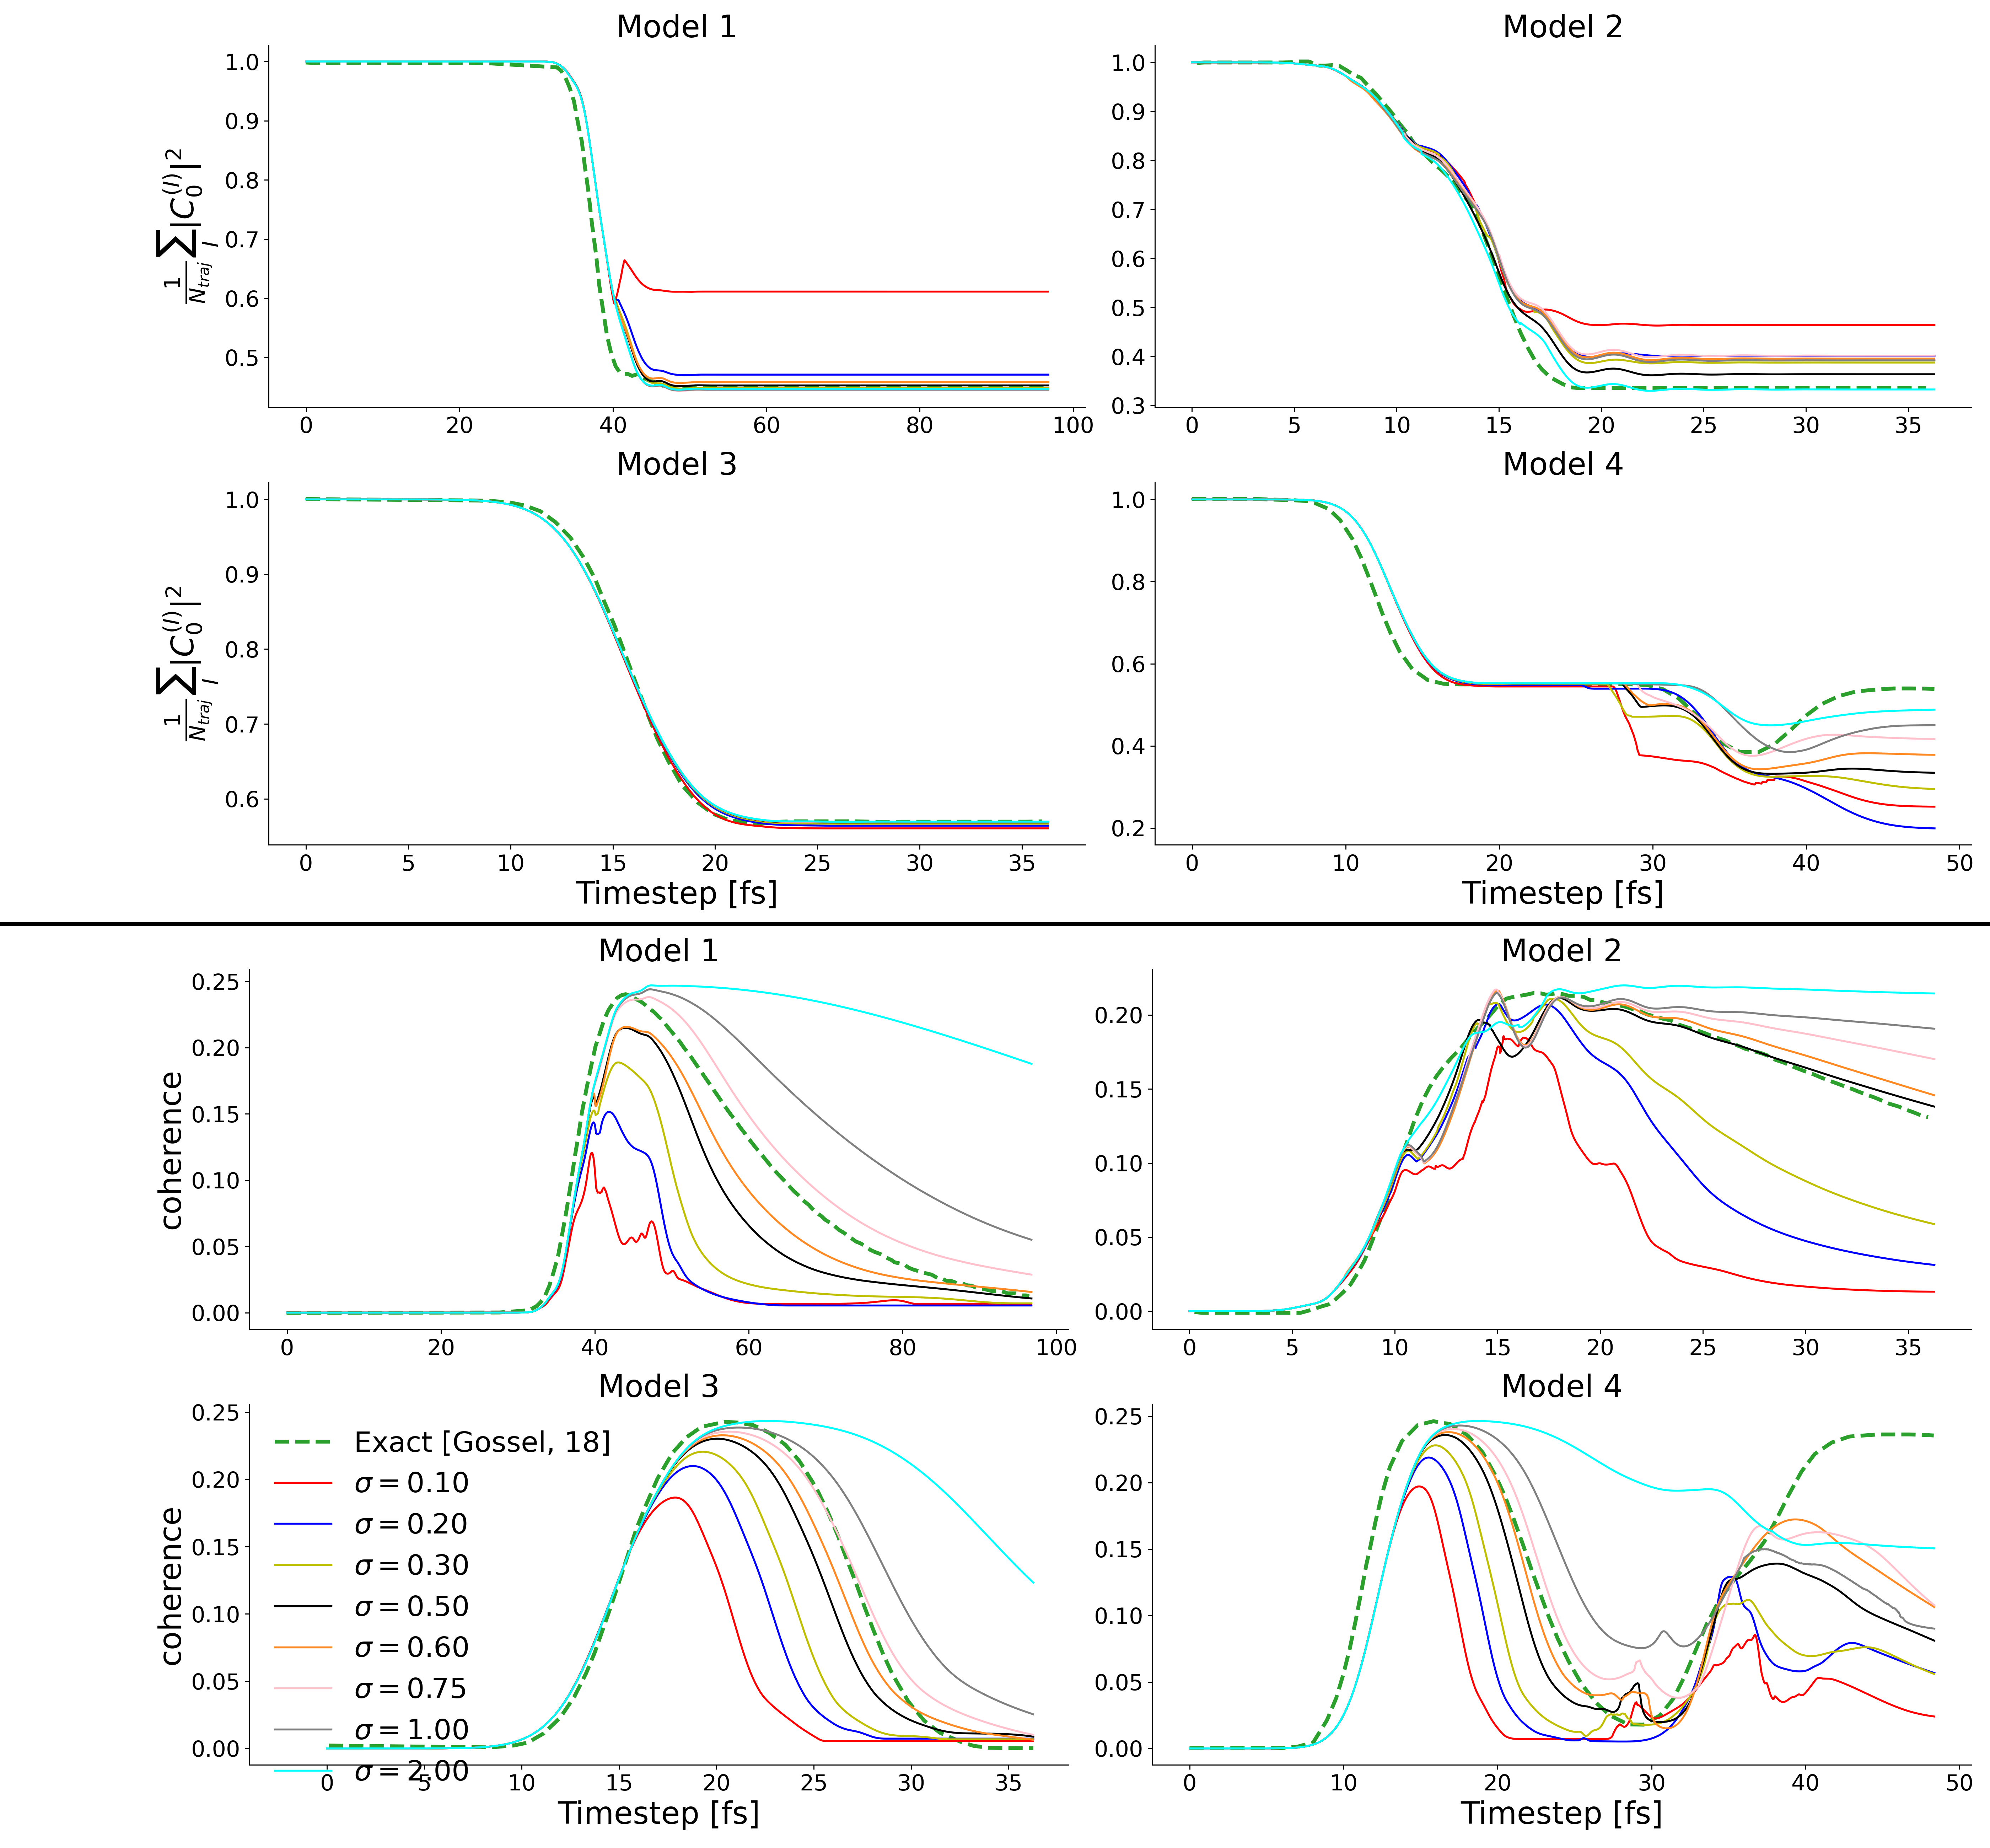
\includegraphics[width=\textwidth]{./img/CTMQC/TullyModels/CTMQC_VarSig_highMom.png}
  \caption{\label{fig:VaryingSigmaTullyModels}4 high momenta cases of the Tully models with a various constant $\sigma$ values used in the calculation of the quantum momentum. Thin solid lines show results from my simulations. The thick, green, dashed line shows data from exact quantum dynamics simulations taken from Gossel \cite{gossel_coupled-trajectory_2018} which should be taken as a reference.}
\end{figure}
\noindent The simplest option for the calculation of $\mathcal{Q}_{lk, \nu}^{(I)}$ is to keep the gaussian width parameter, $\sigma$, constant throughout the simulation. This also allows us to investigate the role of $\sigma$ within the simulations and to determine its influence on the dynamics. To this end various simulations were carried out on the 4 Tully models with the high initial momentum. In each simulation parameters were all the same apart from the value of $\sigma$ which took a value of either: 0.1, 0.2, 0.3, 0.5, 0.6, 0.75, 1 or 2 bohr. The results for these simulations are shown in figure \ref{fig:VaryingSigmaTullyModels}. In this figure, we see that as the $\sigma$ parameter is increased the levels of decoherence also increases. This means for larger $\sigma$ values electronic populations remain in a mixed state for longer and take more time to collapse onto a single adiabatic state. Clearly, the construction of this $\sigma$ parameter is important for recovery of correct electronic dynamics. Surprisingly, this doesn't seem to have much of an effect on the resulting populations. However, this is due to the fact in the limit of large $\sigma$ CTMQC becomes identical to Ehrenfest dynamics and Ehrenfest dynamics captures the evolution of the adiabatic populations very well for each model, with the exception of model 4. It should also be noted that for small values of $\sigma$, propagation using CTMQC can become unstable due to a noisy nuclear density giving rise to an unstable quantum momentum term. A value of 0.6 bohr qualitatively seems to provide the best fit to exact data. However, this may not be appropriate for all types of simulations and a deeper investigation into this parameter would be useful to investigate how general this finding is.

\subsection{Dynamic $\sigma^{(I)}_{\nu}(t)$ calculation}
\begin{figure}[ht]
  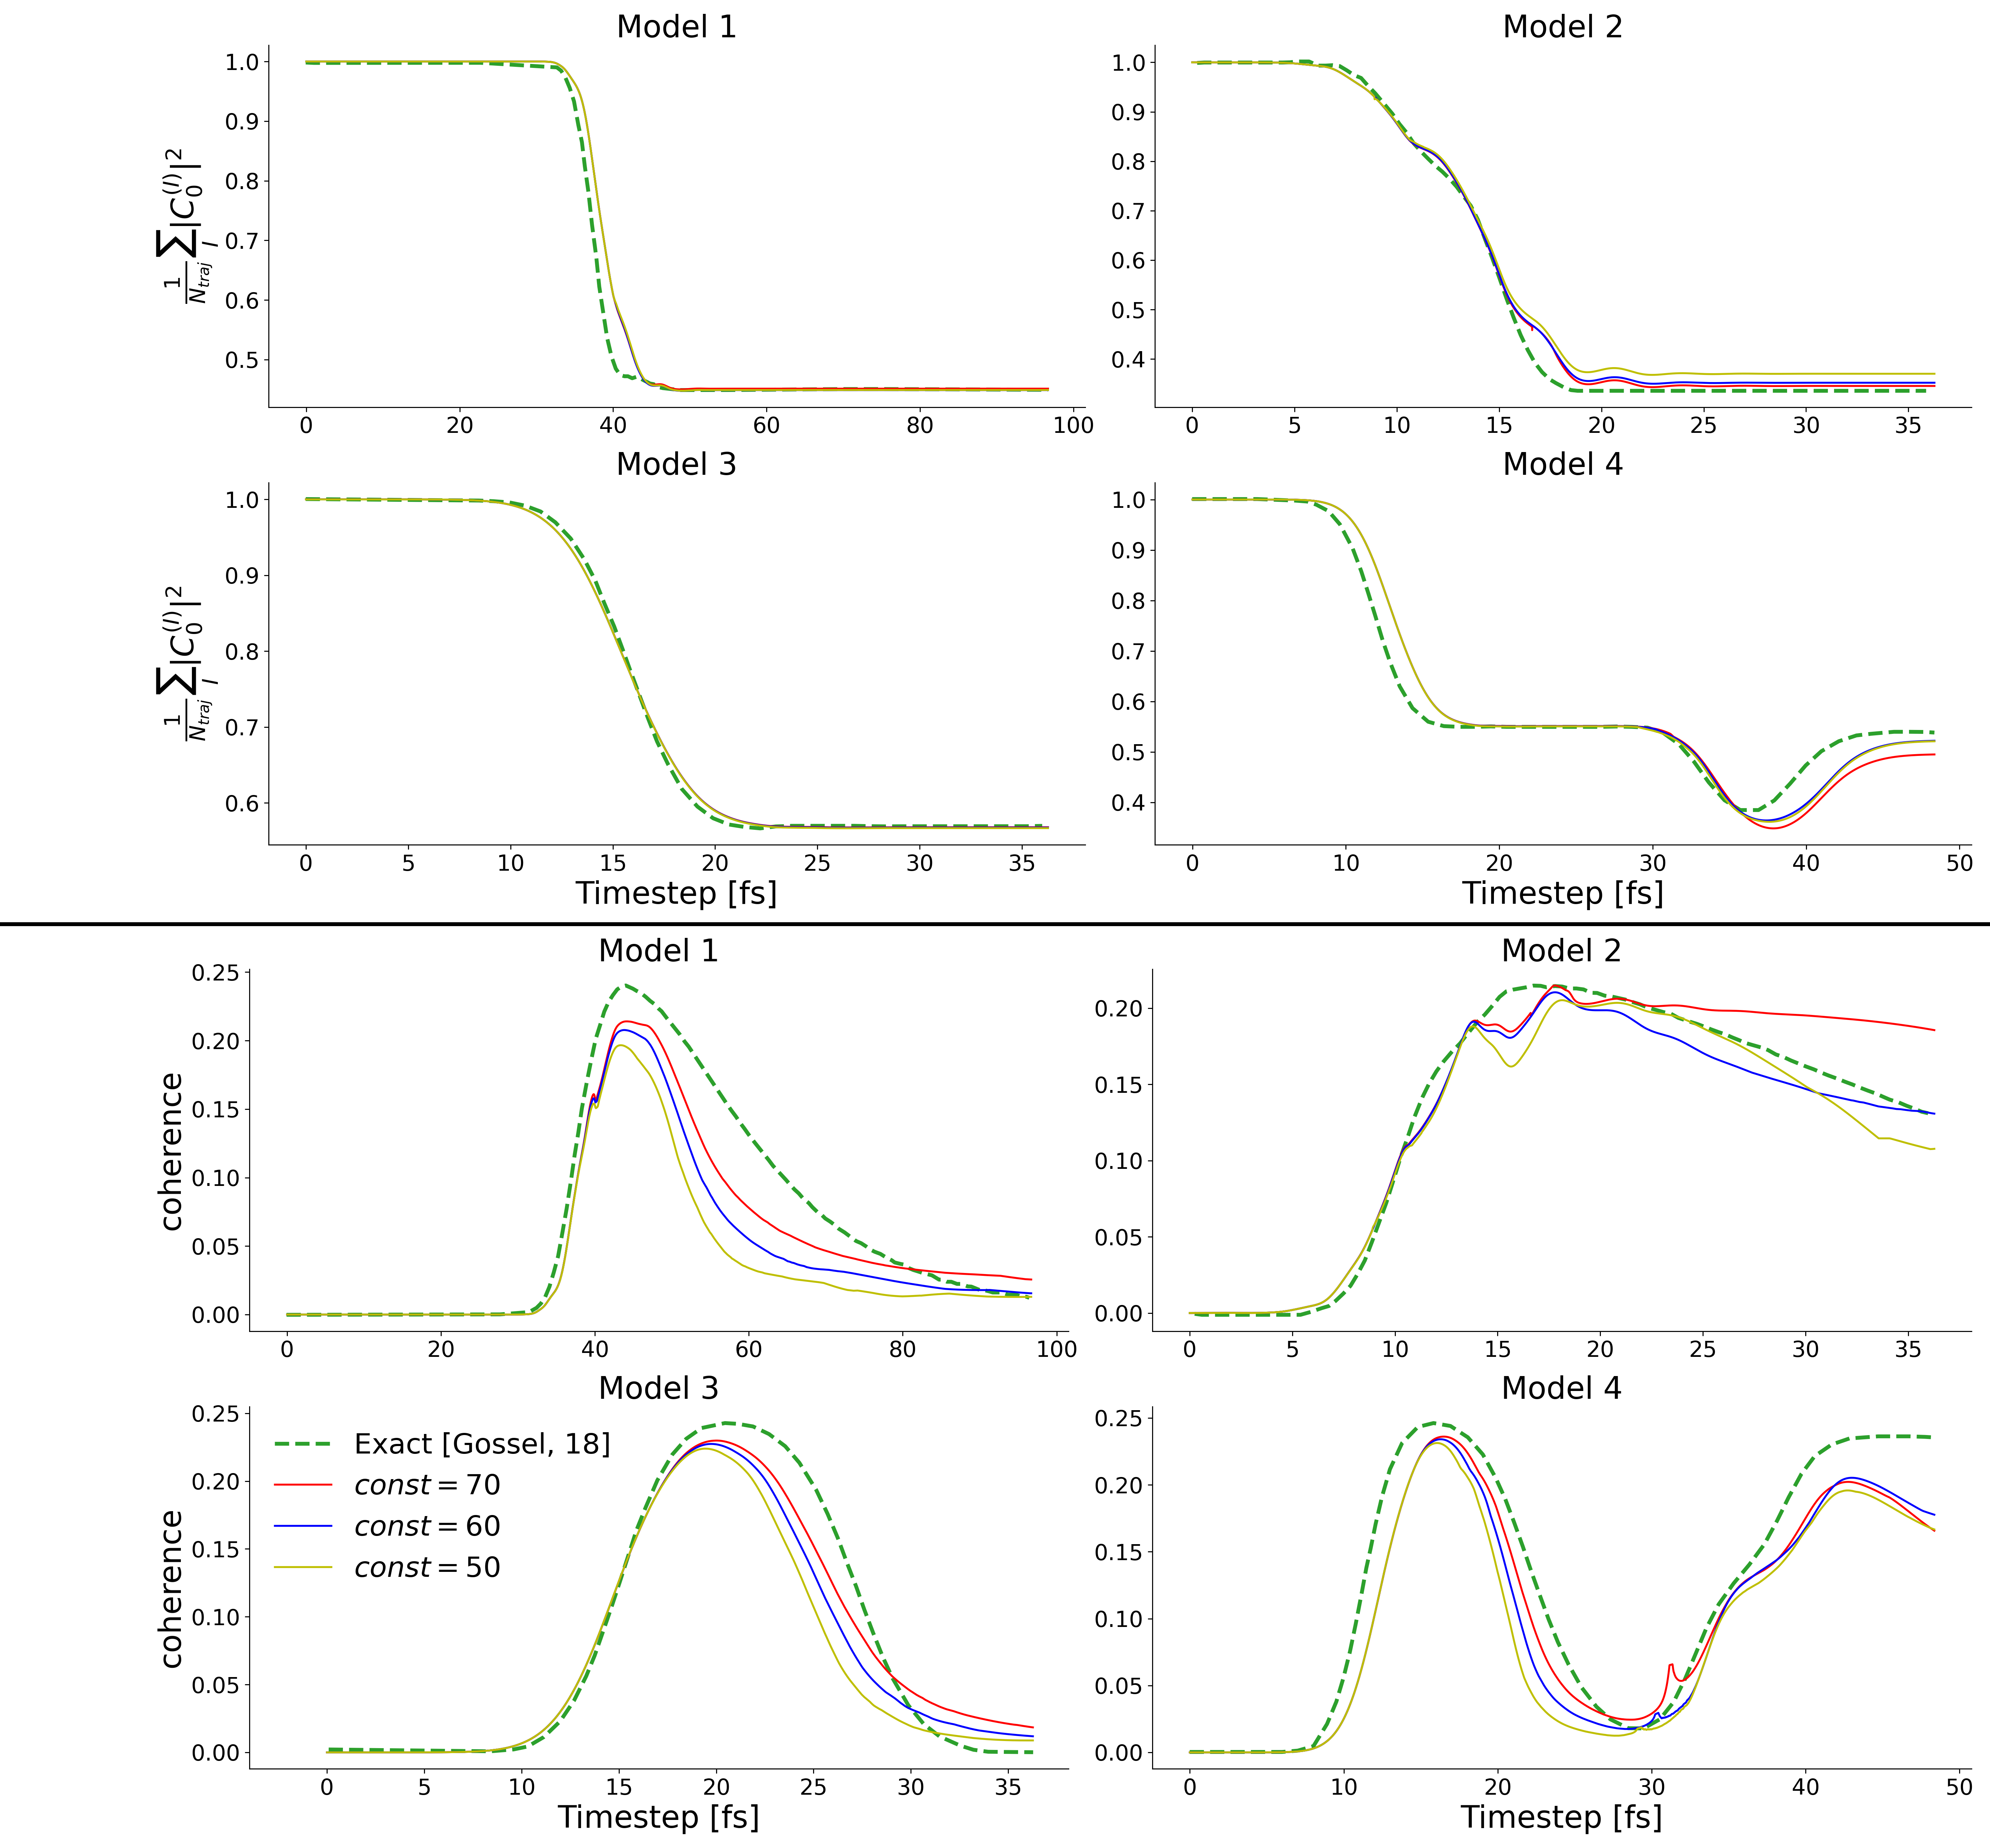
\includegraphics[width=\textwidth]{img/CTMQC/TullyModels/CTMQC_dynSig_highMom.png}
  \caption{\label{fig:dynamicSigma}}
\end{figure}
In the appendix of Gossel \cite{gossel_coupled-trajectory_2018} an algorithm was outlined to calculate $\sigma$ on-the-fly based on the density of replicas within a cutoff distance of each atom. This is given in appendix \ref{ap:DynamicSigma}. However, this method also relies on a constant parameter to calculate $\sigma$ so doesn't remove a parameter, though the resulting dynamics do not seem as sensitive to changes in this parameter as in $\sigma$ itself.
\\\\
Figure \ref{fig:dynamicSigma} shows populations and coherences for the 4 (high momentum) Tully models with various values of const. It is encouraging to see populations now resemble exact results more closely. This is especially true in model 4, where the dip in the populations is recovered. All 3 constants give nearly identical populations, though a constant of 60 seems to give results that most closely resemble the exact coherences. However, seeing as this (like the width parameter) is not a physical parameter it is hard to know if this is reasonable for all systems. 
\section{Conclusion}
In this chapter I have reported results from my implementation of the CTMQC equations applied to the Tully models. The Tully models are a set of 4 Hamiltonians dictating the motion of 1 atom in 1 dimension. These models are commonly simulated as they are simple enough to be solved analytically and complex enough to provide a reasonable test for any new nonadiabatic molecular dynamics (NAMD) technique. I have shown results from various tests which validate my implementation and shown how well CTMQC conserves the norm of the wavefunction and total energy, with the latter showing some concerning results. The reason for this is still unknown. I have also highlighted 2 issues with the dynamics in CTMQC. These are the sudden divergences in the quantum momentum term and the ambiguity surrounding the calculation of the gaussian width parameter, $\sigma$. The former issue has not been discussed in the literature  though I have given a method designed to address it. This has been shown to significantly improve the norm conservation in the Tully model systems. The latter problem has been touched upon in the literature, though no thorough studies have been reported. I have given results for a various values of the gaussian width parameter, $\sigma$, and shown how it can affect the propagation dynamics. Further, I have implemented a method designed to dynamically update the $\sigma$ parameter and benchmarked this against exact quantum dynamics simulations.
\\\\
The propagation of the CTMQC equations using a model Hamiltonian is a good first step in implementing a new NAMD technique. It's relative simplicity allows for a close inspection of each of the quantities involved in the propagation, especially new quantities such as the adiabatic momentum term, $\mathbf{f}_{l, \nu}^{(I)}$ and the quantum momentum term, $\mathcal{Q}_{lk, \nu}^{(I)}$. The same code used to simulate the Tully model system can also be used as a base for future extensions such as in 3D or many atom systems. However, before such extensions are implemented a new way to construct the Hamiltonian is needed. In the next chapter I will discuss my implementation of CTMQC within the fragment orbital based framework which relies on the fast calculation of the Hamiltonian using a finite difference method for off-diagonals and a classical force-field to calculate diagonal terms. 



